\documentclass[oneside,a4paper,14pt]{extreport}

% Font tiếng Việt
\usepackage[T5]{fontenc}
\usepackage[utf8]{inputenc}
\usepackage{amsmath}
\usepackage{amssymb}
\DeclareTextSymbolDefault{\DH}{T1}

% Tài liệu tham khảo
\usepackage[
	sorting=nty,
	backend=bibtex,
  style=numeric]{biblatex}

\usepackage[unicode]{hyperref} % Bookmark tiếng Việt
\addbibresource{References/references.bib}

\makeatletter
\def\blx@maxline{77}
\makeatother

% Chèn hình, các hình trong luận văn được để trong thư mục Images/
\usepackage{graphicx}




% Chèn và định dạng mã nguồn
\usepackage{listings}
\usepackage{color}


% Chèn và định dạng mã giả
\usepackage{amsmath}
\usepackage{algorithm}
\usepackage[noend]{algpseudocode}
\makeatletter
\def\BState{\State\hskip-\ALG@thistlm}
\makeatother

% Bảng biểu
\usepackage{multirow}
\usepackage{array}
\newcolumntype{L}[1]{>{\raggedright\let\newline\\\arraybackslash\hspace{0pt}}m{#1}}
\newcolumntype{C}[1]{>{\centering\let\newline\\\arraybackslash\hspace{0pt}}m{#1}}
\newcolumntype{R}[1]{>{\raggedleft\let\newline\\\arraybackslash\hspace{0pt}}m{#1}}



% Vẽ cây
\usepackage{tikz}
\usetikzlibrary{calc}
\usetikzlibrary{trees}

% Dãn dòng 1.5
\usepackage{setspace}
\onehalfspacing

% Thụt vào đầu dòng
\usepackage{indentfirst}

% Canh lề
\usepackage[
top=30mm,
bottom=25mm,
left=30mm,
right=20mm,
includefoot]{geometry}

% Trang bìa
\usepackage{tikz}
\usetikzlibrary{calc}
\newcommand\HRule{\rule{\textwidth}{1pt}}
% ========================================================================================= %
% PACKAGE CUSTOMIZE
% pdf
\usepackage{pdfpages}

\usepackage[strings]{underscore}
\usepackage{url}

% Math
\usepackage{amsfonts}

\usepackage{stmaryrd}


% Vẽ cây
\usetikzlibrary{trees}

% caption
\usepackage[justification=centering,font=small,labelfont=bf]{caption}
\captionsetup[figure]{font=small}
% % subfigure
\usepackage[font=small,labelfont=bf]{subcaption}
\usepackage{wrapfig}
% \usepackage[justification=centering,font=normalsize]{caption}


\usepackage{tocloft}
\usepackage{tabularx}
\usepackage{booktabs}

% Bảng thuật ngữ
\usepackage[acronym,nomain]{glossaries}

% Customize 
\usepackage[export]{adjustbox}

\usepackage{multicol}

\graphicspath{{images/}}


% ~~~~~~~~~~~~ Custom ~~~~~~~~~~~~
%\usepackage{framed}
\usepackage[capitalise]{cleveref}
\usepackage{algorithm,algorithmicx,algpseudocode}
\usepackage{array}
\usepackage[parfill]{parskip}
%\usepackage{subcaption}
\usepackage{bm}
\usepackage{gensymb}
\usepackage[]{units}
\usepackage{listings}
\usepackage{multicol}
\usepackage{tcolorbox}
% -- \usepackage{physics}
\usepackage{ulem}
% ~~~~~~~~~~~~ Custom ~~~~~~~~~~~~
\graphicspath{{images/}}
\usepackage{hyperref}

\input{Preamble/commands.tex}
% ========================================================================================= %
% CHÚ Ý: Thông tin chung về KLTN - sinh viên điền vào đây để tự động update các trang khác  %
% ========================================================================================= %
\newcommand{\tenSV}{Hoàng~Minh~Thanh} % Dấu ~ là khoảng trắng không được tách (các chữ nối với nhau bằng dấu ~ sẽ nằm cùng 1 dòng
\newcommand{\mssv}{21C11029}
\newcommand{\tenKL}{XÂY DỰNG HỆ THỐNG SINH CỬ CHỈ TỪ ÂM THANH CHO TRỢ LÝ ẢO} % Chú ý dấu ~ trong tên khóa luận
\newcommand{\tenGVHD}{PSG. TS. Lý Quốc Ngọc}
\newcommand{\tenBM}{BM. Khoa~Học~Máy~Tính}

\begin{document}

%\begin{titlepage}
%
%\begin{center}
%%ĐẠI HỌC QUỐC GIA THÀNH PHỐ HỒ CHÍ MINH\\
%TRƯỜNG ĐẠI HỌC KHOA HỌC TỰ NHIÊN\\
%\textbf{KHOA CÔNG NGHỆ THÔNG TIN}\\[2cm]
%
%
%{ \Large \bfseries \tenSV \\[1cm] } 
%
%%Tên đề tài Khóa luận tốt nghiệp/Đồ án tốt nghiệp
%
%{ \Large \bfseries BÁO CÁO KHÓA LUẬN TỐT NGHIỆP \\
%    OpenHuman: Mô hình tổng hợp cử chỉ hội thoại đa phương
%    thức dựa trên văn bản và âm thanh
%%OpenHuman: Multi-modal conversational gestures
%%synthesis based on text and speech 
%\\ [2cm]}
%
%
%%Chọn trong các dòng sau
%\large KHÓA LUẬN TỐT NGHIỆP THẠC SĨ\\
%%\large ĐỒ ÁN TỐT NGHIỆP CỬ NHÂN\\
%%\large THỰC TẬP TỐT NGHIỆP CỬ NHÂN\\
%%Đưa vào dòng này nếu thuộc chương trình Chất lượng cao, hoặc lớp Cử nhân tài năng
%% \large CHƯƠNG TRÌNH THẠC SĨ\\
%% \large CHƯƠNG TRÌNH CHÍNH QUY\\
%%\large CHƯƠNG TRÌNH CHẤT LƯỢNG CAO\\
%%\large CHƯƠNG TRÌNH CỬ NHÂN TÀI NĂNG\\[2cm]
%
%
%\begin{tikzpicture}[remember picture, overlay]
%  \draw[line width = 2pt] ($(current page.north west) + (2cm,-2cm)$) rectangle ($(current page.south east) + (-1.5cm,2cm)$);
%\end{tikzpicture}
%
%\vfill
%Tp. Hồ Chí Minh, tháng 12/2024
%
%\end{center}
%
%\pagebreak
%
%
%
%\begin{center}
%
%TRƯỜNG ĐẠI HỌC KHOA HỌC TỰ NHIÊN\\
%\textbf{KHOA CÔNG NGHỆ THÔNG TIN}\\[2cm]
%
%
%{\large \bfseries Hoàng Minh Thanh - 21C11029\\[2cm]}
%
%%Tên đề tài Khóa luận tốt nghiệp/Đồ án tốt nghiệp
%
%{ \Large \bfseries  BÁO CÁO KHÓA LUẬN TỐT NGHIỆP \\ 
%    OpenHuman: Mô hình tổng hợp cử chỉ hội thoại đa phương
%    thức dựa trên văn bản và âm thanh
%%	HỆ THỐNG TỔNG HỢP CỬ CHỈ DỰA TRÊN VĂN BẢN VÀ ÂM THANH
%    \\[2cm] } 
%
%
%%Chọn trong các dòng sau
%\large KHÓA LUẬN TỐT NGHIỆP THẠC SĨ \\
%
%%\large ĐỒ ÁN TỐT NGHIỆP CỬ NHÂN\\
%%Đưa vào dòng này nếu thuộc chương trình Chất lượng cao, hoặc lớp Cử nhân tài năng
%% \large CHƯƠNG TRÌNH HOÀN CHỈNH\\[2cm]
%%\large CHƯƠNG TRÌNH CHẤT LƯỢNG CAO\\[2cm]
%%\large CHƯƠNG TRÌNH CỬ NHÂN TÀI NĂNG\\[2cm]
%
%\textbf{GIÁO VIÊN HƯỚNG DẪN}\\
%\tenGVHD\\
%\tenBM\\
%
%\begin{tikzpicture}[remember picture, overlay]
%  \draw[line width = 2pt] ($(current page.north west) + (2cm,-2cm)$) rectangle ($(current page.south east) + (-1.5cm,2cm)$);
%\end{tikzpicture}
%
%\vfill
%Tp. Hồ Chí Minh, tháng 12/2024
%
%\end{center}
%
%\end{titlepage}


\begin{mdframed}[linewidth=1pt, % Độ dày của viền
	linecolor=black, % Màu của viền
	leftmargin=0, % Khoảng cách lề trái
	rightmargin=0, % Khoảng cách lề phải
	innertopmargin=20mm, % Khoảng cách lề trên trong
	innerbottommargin=20mm, % Khoảng cách lề dưới trong
	innerleftmargin=25mm, % Khoảng cách lề trái trong
	innerrightmargin=25mm, % Khoảng cách lề phải trong
	skipabove=0, % Khoảng trắng trước khung
	skipbelow=0] % Khoảng trắng sau khung
	\centering
	\vspace*{1cm}
	
	{\fontsize{13}{15}\selectfont{ ĐẠI HỌC QUỐC GIA TP. HCM}}\\
	\vspace{0.25cm}
	{\fontsize{13}{15}\selectfont\textbf{TRƯỜNG ĐẠI HỌC KHOA HỌC TỰ NHIÊN}}\\
	
	\vspace{3cm}
	
	{\fontsize{14}{16}\selectfont\textbf{HOÀNG MINH THANH}}\\
	
	\vspace{3cm}
	
	{\fontsize{14}{16}\selectfont\textbf{\MakeUppercase{OPENHUMAN: MÔ HÌNH TỔNG HỢP CỬ CHỈ HỘI THOẠI ĐA PHƯƠNG THỨC DỰA TRÊN VĂN BẢN VÀ ÂM THANH}}}\\
	
	\vspace{3cm}
	
	{\fontsize{14}{16}\selectfont\textbf{LUẬN VĂN THẠC SĨ}}\\
	
	\vfill
	
	\vspace{3cm}
	
	{\fontsize{13}{15}\selectfont TP. Hồ Chí Minh – Năm 2024}
\end{mdframed}

\pagenumbering{gobble}  
\pagebreak

\begin{mdframed}[linewidth=1pt, 
	linecolor=black, 
	innerleftmargin=10mm, 
	innerrightmargin=10mm, 
	innertopmargin=10mm, 
	innerbottommargin=10mm]
	\centering
	\vspace*{1cm}
	
	\Large ĐẠI HỌC QUỐC GIA TP. HCM\\
	\vspace{0.25cm}
	\Large \textbf{TRƯỜNG ĐẠI HỌC KHOA HỌC TỰ NHIÊN}\\
	
	\vspace{2cm}
	
	\Large HOÀNG MINH THANH \\
	
	\vspace{3cm}
	
	\Large \textbf{\MakeUppercase{OPENHUMAN: MÔ HÌNH TỔNG HỢP CỬ CHỈ HỘI THOẠI ĐA PHƯƠNG THỨC DỰA TRÊN VĂN BẢN VÀ ÂM THANH}}\\
	
	\vspace{1cm}
	
	\flushleft
	{\fontsize{13}{15}\selectfont Ngành: Khoa học máy tính}\\
	{\fontsize{13}{15}\selectfont Mã số Ngành: 8480101}\\
	
	\vspace{3cm}
	
	\centering
	\Large NGƯỜI HƯỚNG DẪN KHOA HỌC\\
	\Large HDC: PSG. TS. LÝ QUỐC NGỌC \\
	
	\vfill
	\vspace{3cm}
	
	{\fontsize{12}{13} TP. Hồ Chí Minh – Năm 2024}
\end{mdframed}



\pagenumbering{gobble}  
\pagebreak
\pagenumbering{roman}


\pagebreak

% Sasu trang Title, các bạn chèn nhận xét gủa GVHD và GVPB. Nhận xét sẽ được giáo vụ phát sau buổi bảo vệ để các bạn đóng quyển.

\pagenumbering{roman} % Đánh số i, ii, iii, ...

\addcontentsline{toc}{chapter}{Lời cam đoan}

\section*{\centering  LỜI CAM ĐOAN}
\phantomsection
\addcontentsline{toc}{section}{Lời cam đoan}


{
Tôi cam đoan luận văn thạc sĩ ngành Khoa học máy tính, với đề tài OpenHuman: Mô hình tổng hợp cử chỉ hội thoại đa phương thức dựa trên văn bản và âm thanh là công trình khoa học do tôi thực hiện dưới sự hướng dẫn của TS. Lý Quốc Ngọc, những kết quả nghiên cứu của luận văn hoàn toàn trung thực và chính xác.

Bản quyền toàn bộ các sản phẩm của luận văn này thuộc về thầy Lý Quốc Ngọc và Trường Đại học Khoa học tự nhiên. Tôi sẽ không sử dụng chúng ở những nơi khác, với bất kỳ mục đích nào khác.



\begin{table}[h]
    \centering
        \begin{tabular}{p{7cm}p{7cm}}
        \textbf{\begin{tabular}[c]{@{}c@{}}\\\\\\ \textit{}\end{tabular}} & \textbf{\begin{tabular}[c]{@{}c@{}}\textit{TP. Hồ Chí Minh, ngày... tháng... năm...}\\HỌC VIÊN THỰC HIỆN\\\textit{(Ký và ghi rõ họ tên}) \end{tabular}}
        \end{tabular}
    \end{table}
    }
    \pagebreak

\pagebreak

\addcontentsline{toc}{chapter}{Lời cảm ơn}
\include{Appendix/thanks}

\addcontentsline{toc}{chapter}{Đề cương chi tiết}
%\include{Appendix/decuong}

% Mục lục, danh sách hình, danh sách bảng
\addcontentsline{toc}{chapter}{Mục lục}
\tableofcontents
\listoffigures
\listoftables

\addcontentsline{toc}{chapter}{Tóm tắt}
\chapter*{Tóm tắt}
\label{abstract}

Xây dựng người kỹ thuật số (digital human) hay các nhân vật trợ lý ảo siêu thật có thể tương tác như một con người là mục tiêu nghiên cứu từ lâu của các nhà khoa học máy tính. Với sự phát triển của đồ họa máy tính trong việc mô phỏng người siêu thật cũng như sự phát triển mạnh mẽ của phần cứng máy tính và thành công của các mô hình ngôn ngữ lớn gần đây.
Thì nút thắt cổ chai duy nhất hiện nay là việc sinh ra các biểu cảm khuôn mặt (facial expression), cũng như các khung xương (joins) 3D trước khi kết xuất (render) để hiển thị lên màn hình cho người dùng.
Sinh cử chỉ (gesture generation) không chỉ được sử dụng để xây dựng người trợ lý ảo mà còn được sử dụng trong game, robot cũng như trong công nghiệp điện ảnh.
Để giải quyết vấn đề đồng bộ giữa âm thanh và cử chỉ, chúng tôi đề xuất phương pháp \textbf{OHGesture} dựa trên mô hình diffusion với đầu vào là chuỗi cử chỉ khởi tạo, và đoạn âm thanh tương ứng.
Đóng góp của tôi là sử dụng văn bản và cảm xúc, sử dụng cơ chế cross-attention và self-attention trong quá trình diffuse để sinh cử mượt mà và chân thực.

Thực nghiệm chứng minh phương pháp của chúng tôi có thể giúp chúng tôi tạo ra cử chỉ theo nhiều cảm xúc khác nhau và đạt kết quả tốt hơn khi áp dụng cross-attention.

% Ngoài ra mô hình OHGesture cũng sinh được các cử chỉ với đa dạng cảm xúc khác nhau như vui vẻ, buồn bã, người già.

% OHGesture sẽ biểu diễn các dự liệu đầu vào thành các vùng trong không gian với mỗi vùng một đại diện tương ứng. Sau đó sắp xếp lại vị trí đại diện của mỗi vùng dựa trên khoảng cách với cử chỉ khởi tạo để tạo ra các chuỗi cử chỉ ứng viên.

% Cử chỉ sinh ra do người nói có tính tuần hoàn, dựa vào phương pháp mã hóa tuần hoàn (Periodic Autoencoders \cite{starke2022deepphase} ), mô hình sẽ trích xuất được các pha (phrase) của cử chỉ, từ đó giúp mô hình chọn được cử chỉ có pha phù hợp với ngữ nghĩa hoặc nhịp điệu của lời nói.
% Đóng góp của chính của chúng tôi là 

Mã nguồn của chúng tôi mà mô hình pre-train và minh họa ở

\href{https://github.com/hmthanh/OHGesture}{hmthanh/OHGesture}

\clearpage

\pagenumbering{arabic} % Đánh số 1, 2, 3, ...

% Các chương nội dung
% Giới thiệu
% \usepackage[utf8]{inputenc}
% \usepackage[T1]{fontenc}%❖ Là chương mở rộng của tóm tắt
%❖ Nội dung bao gồm
%o Ngữ cảnh, vấn đề cần giải quyết là gì?
%o Vì sao vấn đề/bài toán quan trọng và thú vị?
%o Bài toán có gì khó? Vì sao cần phải giải quyết?
%o Những giải pháp (nghiên cứu, ứng dụng) đã giải quyết bài toán này?
%o Những giải pháp này có hạn chế, thiếu sót gì?
%o Giải pháp của bạn là gì? Kết quả thế nào?
%o Đóng góp của nghiên cứu/ứng dụng của bạn? 
%❖ Độ dài từ 3 đến 8 trang
%❖ Có thể chia ra các mục
%o Đặt vấn đề (Problem)
%o Mục tiêu (Objectives)
%o Giải pháp/Cách tiếp cận (An Approach)
%o Đóng góp (Contributions)
%o Bố cục (Outline)
%❖ Lưu ý, nội dung các chương sau phải khớp với mục tiêu, giải pháp, đóng góp ở chương này
\chapter{Giới thiệu}
\label{Chapter1}

\section{Bối cảnh chung}

\begin{figure}[h!]
  \centering
  \includegraphics[width=0.5\linewidth]{images/cgi.png}
  \caption{Công nghệ CGI với người kỹ thuật số siêu thật}
  \label{fig:cgi}
\end{figure}

Mỗi ngày, trên thế giới có hàng tỷ người nhìn vào màn hình RGB, kết quả hiển thị trên màn hình là đầu ra của mọi hệ thống phần mềm, nên việc hiển thị từng pixel trên màn hình và cách để mô phỏng lại hình ảnh trên một cách chân thực nhất được các nhà khoa học về đồ họa máy tính (Computer Graphic) nghiên cứu từ những năm 1960s và đặc biệt là việc mô phỏng lại con người \autoref{fig:cgi}. 

Ngày nay, công nghệ đồ họa máy tính đã hoàn toàn có thể mô phỏng nhiều vật giống đến mức siêu thực (realistic) các vật phức tạp như nước, đường xá, bánh mỳ,...  và thậm chí là cả cơ thể và khuôn mặt con người với độ chi tiết đến từng lông tơ, nốt mụn và vân mắt. 
Vào năm 2015, bằng kỹ thuật quyét 3 chiều ghi lại toàn bộ các góc của khuôn mặt, sự phản chiếu ánh sáng, trong công trình \cite{metallo2015scanning}
nhà khoa học đồ họa máy tính đã có thể tái tạo toàn bộ khuôn mặt của tổng thống Obama trên máy tính với độ chính xác cao và gần như không thể phân biệt \autoref{fig:obamascan}.

\begin{figure}
    \centering
    \includegraphics[width=\linewidth]{images/obama_scan.jpg}
    \caption{Minh họa công trình tái tạo khuôn mặt tổng thống Obama}
    \label{fig:obamascan}
\end{figure}

Trí tuệ nhân tạo thể hiện kết quả vượt bậc những năm gần đây không chỉ trong nghiên cứu mà con trong ứng dụng thực tế, tiêu biểu như ứng dụng ChatGPT, Midjouney và sự phát triển cả theo chiều dọc và chiều ngang trong việc ứng dụng trí tuệ nhân tạo với nhiều lĩnh vực khác nhau. Mặc dù đồ họa máy tính đã có thể xây dựng khuôn mặt người siêu thật, việc sinh cử chỉ lại phụ thuộc vào việc Chụp chuyển động (Motion Capture) từ các cảm biến và gặp rất nhiều khó khăn khi xây dựng một hệ thống trí tuệ nhân tạo để học từ dữ liệu.

Các hệ thống trí tuệ nhân tạo hiện nay đã có thể tạo văn bản và âm thanh tiệm cận như con người, nhưng một trong những trở ngại lớn nhất để xây dựng con người kỹ thuật số hiện nay chính là việc sinh cử chỉ. Chính vì vậy mà mục tiêu của luận văn là xây dựng một hệ thống sinh cử chỉ hội thoại dựa trên cảm xúc và ngữ nghĩa với dữ liệu đầu vào gồm cả văn bản và giọng nói.

\section{Động lực nghiên cứu}

% Ý nghĩa khoa học và ứng dụng của đề tài
% Vai trò của việc sinh cử chỉ
Tổng hợp cử chỉ hội thoại giúp ích cho rất nhiều lĩnh vực như hoạt ảnh, dựng phim, trò chơi điện tử, giáo dục và những ứng dụng thực tại ảo. Việc tổng hợp cử chỉ chuyển động được thực hiện theo cách truyền thống là thuê các diễn viên sử dụng các tracker và bố trí các hệ thống cảm biến xung quanh thu nhận chuyển động để đạt được độ chính xác nhân thực nhất. Tuy nhiên, các chuyển động thu được sau đó chỉ được phát lại và không có sự biến chuyển giữa các hành động hay chuyển động, chính vì vậy, việc áp dụng trí tuệ nhân tạo để có thể học các chuyển động từ dữ liệu thu nhận và sau đó có thể sinh ra dữ liệu mới sẽ là một cuộc cách mạng trong ngành công nghiệp Motion Capture.

Vào năm 2011, một nhóm tác giả \cite{bergmann2011relation} đã chứng minh rằng có sự liên hệ giữa giọng nói và cử chỉ con người, đây chính là tiền đề để cho thấy chúng ta có thể dùng dữ liệu âm thanh để có thể dùng để học và biểu diễn được cử chỉ con người.
Với sự thành công của các mô hình ngôn ngữ tự nhiên trong việc xử lý ngôn ngữ văn bản, với sự chính xác siêu thật trong việc mô phỏng gương mặt con người trong lĩnh vực Đồ họa máy tính và với sự chính xác và dễ dàng từ việc tổng hợp giọng nói con người hiện nay. Thì việc ứng dụng trí tuệ nhân tạo để sinh cử chỉ con người là một trong những điểm nghẽn cổ chai duy nhất trong việc phát triển một trợ lý ảo để trao đổi và tương tác với con người.

\section{Phát biểu bài toán}

Mục tiêu của việc sinh cử chỉ (gesture generation) bằng phương pháp học máy là tạo ra các cử chỉ tự nhiên, chân thật như con người và đồng thời phù hợp với ngữ cảnh.
%Sinh cử chỉ (gesture generation) là bài toán dựa vào những dữ liệu trước đó bao gồm văn bản và âm thanh, cử chỉ khởi tạo để nội suy ra chuỗi cử chỉ tiếp theo.
Sinh cử chỉ là bài toán hồi quy (regression), với đầu vào là một chuỗi cử chỉ cho trước và kết quả đầu ra là chuỗi cử chỉ tiếp tục với cử chỉ trước đó.


\begin{figure}[htbp]
	\centering
	\begin{subfigure}{0.49\textwidth}
		\centering
		\includegraphics[height=10cm]{images/Skeleton.png}
		\caption{\small Khung xương và tên của các khớp của một khung xương trong mỗi khung hình.}
		\label{fig:Skeleton}
	\end{subfigure}
	\hfill
	\begin{subfigure}{0.49\textwidth}
		\centering
		\includegraphics[height=10cm]{images/MotionPastAndFuture.png}
		\caption{\small Chuỗi chuyển động của cử chỉ bao gồm 6 cử chỉ quá khứ và 6 cử chỉ tương lai.}
		\label{fig:MotionPastAndFuture}
	\end{subfigure}
\end{figure}

Mỗi khung hình chuyển động của một nhân vật hay khung xương (skeleton) bao gồm dữ liệu về toạ độ vị trí và vận tốc theo thời gian.
Ở đây dữ liệu của chúng tôi của một khung xương với mỗi khung hình (frame) bao gồm:

\begin{equation} \label{eq:gesturevector}
\mathbf{g} = \Big[ \mathbf{p}_{\text{root}},  \mathbf{r}_{\text{root}},
\mathbf{ p }'_{\text{root}},  \mathbf{r}'_{\text{root}},
\mathbf{p}_{\text{joins}},  \mathbf{r}_{\text{joins}},
\mathbf{p}'_{\text{joins}},  \mathbf{r}'_{\text{joins}},
\mathbf{d}_{\text{gaze}}
\Big]
\end{equation}



Trong  đó với mỗi $\mathbf{g} \in \mathbb{R}^{1141}$ bao gồm:
{
	\small

\begin{itemize}
	\item $\mathbf{p}_{\text{root}} \in \mathbb{R}^3$: Toạ độ của điểm gốc
	\item $\mathbf{r}_{\text{root}} \in \mathbb{R}^4$: Góc quay của điểm gốc
	\item $\mathbf{p}'_{\text{root}} \in \mathbb{R}^3$: Vận tốc thay đổi của toạ độ gốc
	\item $\mathbf{r}'_{\text{root}} \in \mathbb{R}^3$: Vận tốc thay đổi của góc quay gốc
	
	\item $\mathbf{p}_{\text{joins}} \in \mathbb{R}^{3 n_{\text{join} }}$: Toạ độ của các khung xương
	\item $\mathbf{r}_{\text{joins}} \in \mathbb{R}^{3 n_{\text{join} }}$: Góc quay của các khung xương
	\item $\mathbf{p}'_{\text{joins}} \in \mathbb{R}^{3n_{\text{join} }}$: Vận tốc thay đổi của toạ độ các khung xương
	\item $\mathbf{r}'_{\text{joins}} \in \mathbb{R}^{3n_{\text{join} }}$: Vận tốc thay đổi của góc quay các khung xương
	
	\item $\mathbf{d}_{\text{gaze}} \in \mathbb{R}^3$: Là hướng nhìn
\end{itemize}}


%\begin{figure}
%	\centering
%	\includegraphics[width=0.8\linewidth]{images/skeleton_sample.png}
%	\caption{Minh họa một cử chỉ và mô hình nhân vật}
%	\label{fig:software}
%\end{figure}


Tổng cộng có $75$ khớp (joins) hay $n_{\text{join}} = 75$, với mỗi khung hình (frame) ta sẽ có một vector gồm 1141 chiều.
Tập dữ liệu là tập nhiều chuỗi cử chỉ với độ dài tuỳ ý, từ mỗi cử chỉ độ dài tuỳ tý ta sẽ cắt thành các đoạn $8 + N$ khung hình, $g \in \mathbb{R}^{(8+N) \times 1141}$ , trong đó cử chỉ $g \in \mathbb{R}^{8 \times 1141}$ đầu tiên là cử chỉ khởi tạo (seed gesture), $g \in \mathbb{R}^{N \times 1141}$ cử chỉ tiếp theo cho việc dự đoán.


Dữ liệu âm thanh $\mathbf{a}_{\text{raw}} \in \mathbb{R}^{ \text{length } }$  là một chuỗi waveform có độ dài tương ứng với cử chỉ được đọc với sample rate là 16000. 

\begin{figure}
	\centering
	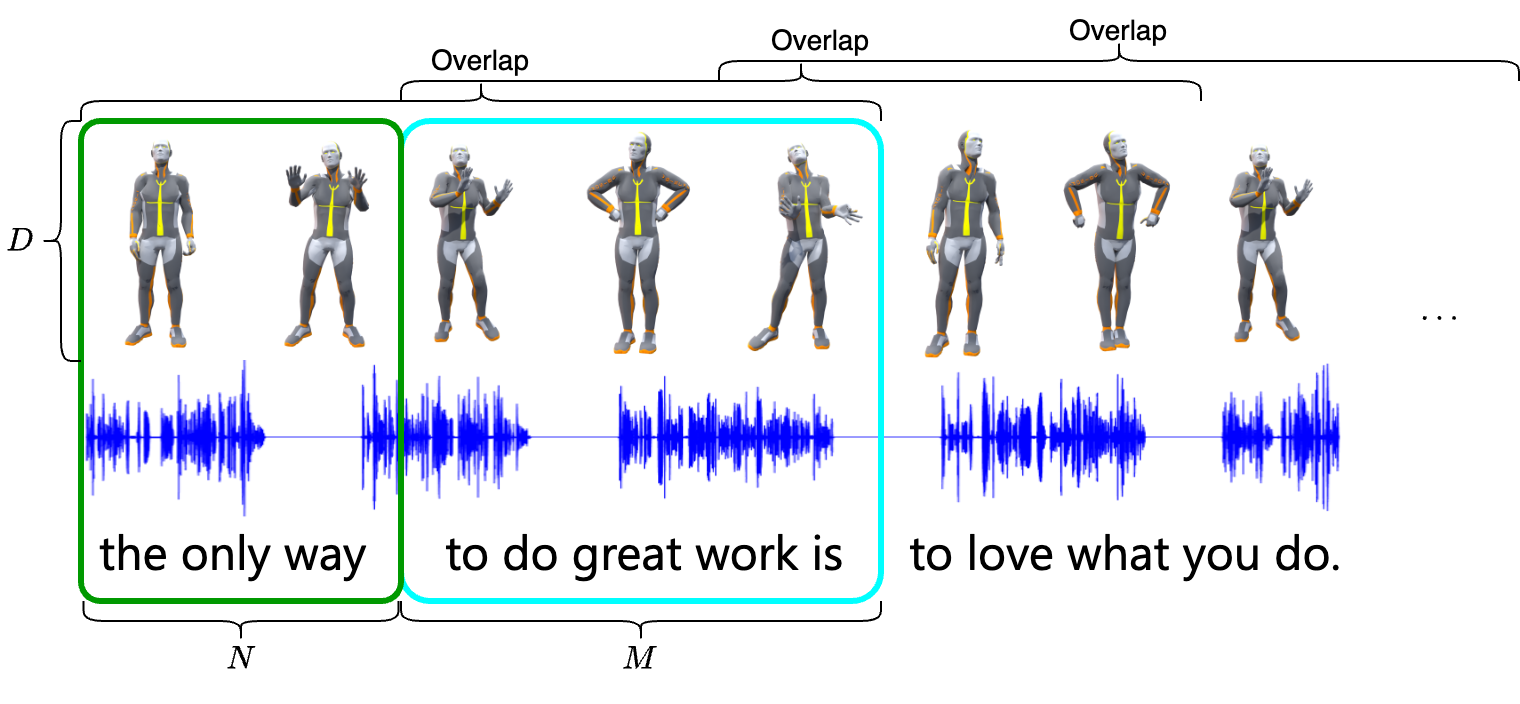
\includegraphics[width=\linewidth]{GestureSeries}
	\caption{Minh hoạ một chuỗi cử chỉ, ta lấy $N$ frame đầu làm cử chỉ khởi tạo $s$ (seed gesture) và $M$ khung hình còn lại làm cử chỉ để học}
	\label{fig:GestureSeries}
\end{figure}


%Chuỗi waveform sẽ được cắt thành các đoạn chồng nhau, áp dụng Hamming windows, và áp dụng thuật toán fast fourier transform để biến đổi chuỗi âm thanh thành các hệ số thể hiện cường độ của các tần số trong chuỗi âm thanh, các hệ số này được làm tròn thành các đoạn tần số (frequency bins), các đoạn hệ số này được chuẩn hoá theo hệ cơ số log để tương ứng với cảm nhận của tai người để có được đặc trưng MFCC $\mathbf{a} \in \mathbb{R}^{\text{size} \times \mathcal{C}}$ trong đó $\mathcal{C}=13$ là số frequency bins. 


% \begin{figure}
%     \centering
%     \includegraphics[width=3cm]{images/gesture_sample.png}
%     \caption{Minh họa cử chỉ}
%     \label{fig:gesture_sample}
% \end{figure}

\section{Các khó khăn cần giải quyết}

Có rất nhiều khó khăn trong việc xây dựng một mô hình có thể học được các đăng trưng cử chỉ hội thoại như con người theo thời gian thực:

Thứ nhất, \textit{dữ liệu không đủ nhiều và chất lượng}, chi phí để tạo ra một bộ dữ liệu trong ngành công nghiệp Motion Capture có chất lượng và quy mô lớn để ứng dụng vào trong thực tế là rất lớn.

Thứ hai, \textit{sự thiếu đồng nhất của về ngữ cảnh của các loại dữ liệu}, các bộ dữ liệu về văn bản thường rất nhiều hơn so với giọng nói và cũng không thể biết được văn bản đó được tạo bởi người nào, sự đồng bộ giữa giọng nói và cảm xúc lúc nói cũng thiếu trong việc tạo tập dữ liệu. Ngoài ra, các dữ liệu văn bản lại được nói bởi rất nhiều người khác nhau và ở nhiều nội dung và chủ đề khác nhau.
 
Thứ ba, \textit{sự phân bố không cân xứng về  dữ liệu giữa các loại đăng trưng cần học}. Các dữ liệu dùng cho nghiên cứu cử chỉ hiện nay thường tập trung vào ngôn ngữ Tiếng Anh, các cử chỉ có sự phân bố không cân xứng giữa khi nói, khi hỏi, khi im lặng.

Thứ tư, \textit{chi phí tính toán với nhiều loại dữ liệu của mô hình rất lớn}. Với đầu vào của mô hình gồm rất nhiều loại dữ liệu khác nhau như văn bản, tiếng nói và điểm 3D, nên cần rất nhiều lớp encode cho từng loại dữ liệu cũng là rào cản không nhỏ bởi chi phí tính toán khi huấn luyện và khi suy luận. Nếu giảm thông tin dữ liệu đầu vào cũng sẽ giảm kết quả suy luận của mô hình khi sinh cử chỉ.

Cuối cùng, \textit{các bước xử lý phải yêu cầu tuần tự}, cách hiệu quả nhất để con người tương tác với máy tính là thông qua giọng nói và nhập từ bàn phím, tuy nhiên việc xử lý được văn bản và giọng nói để làm đầu vào cho mô hình phải thực hiện tuần tự, độ trễ để có thể suy luận trong sản phẩm thực tế cũng là một vấn đề bởi người dùng không thể đợi lâu để nhận được kết quả cử chỉ và từ cử chỉ đó biểu diễn lên máy tính bằng kỹ thuật đồ họa máy tính.

\begin{figure}
	\centering
	\includegraphics[width=\linewidth]{MotionCapture}
	\caption{Khung chương trình xây dựng hệ thống sinh cử chỉ}
	\label{fig:MotionCapture}
\end{figure}

\section{Đóng góp của chúng tôi}

\begin{itemize}
\item Chúng tôi mở rộng mô hình diffusion với thông tin thời gian cho việc sinh cử chỉ kèm theo lời nói dựa trên âm thanh. Nhờ mô hình diffusion, chúng tôi có thể kiểm soát một cách linh hoạt cử chỉ được sinh ra, ví dụ: chỉnh sửa phong cách của cử chỉ, thiết lập cử chỉ khởi tạo, và sinh cử chỉ đa dạng.

\item Chúng tôi sử dụng cross-local attention và self-attention để để học được bối cảnh và những quan hệ giữa cử chỉ và lời nói.

\item Các thử nghiệm mở rộng chỉ ra rằng mô hình của chúng tôi có thể sinh ra cử chỉ giống người, phù hợp với lời nói (speech-appropriateness), phù hợp với cảm xúc (style-appropriateness) vượt trội so với các phương pháp sinh cử chỉ hiện có.
\end{itemize}


% Đầu vào của hệ thống trí tuệ nhân tạo cho việc sinh cử chỉ bao gồm: 

% Tức đã có input (audio/text) sang output (text). Nhưng chưa có từ text sang 1 visual.

% Để xây dựng 1 virtual human assitant mà tương tác được cần sinh ra Output:

% - Hình ảnh: text to visual: 3D scan da người, các texture, mesh và quan trọng nhất là cử chỉ của người đó.

% - Âm thanh: text to speech.

% Để học được các cử chỉ thì dữ liệu đầu vào dĩ nhiên bao gồm các keypoint 3D về cử chỉ, dữ liệu cử chỉ bao gồm cử chỉ của cơ thể ($\Omega_{\text{Body}}$) cử chỉ của bàn tay ($\Omega_{\text{Hand}}$) và biểu cảm khuôn mặt ($\Omega_{\text{Facial}}$).

% $$
% \Omega = \{ \Omega_{\text{Speaker_ID}}; \Omega_{\text{Emotion_ID}}; \Omega_{\text{Text}}; \Omega_{\text{Speech}}; \\
% \Omega_{\text{Facial}}; \Omega_{\text{Hand}}; \Omega_{\text{Body}}
% \} 
% $$

% \section{Bài toán sinh cử chỉ}

%Đầu vào của mô hình sinh cử chỉ là chuỗi văn bản (text), chuỗi lời nói (speech) và tọa độ cử chỉ khởi tạo, với đầu ra là chuỗi cử chỉ được sinh ra tương ứng với văn bản và lời nói tương ứng.

%là các keypoint chuyển động trên không gian tọa độ 3 chiều của cử chỉ cơ thể (\textbf{body gesture}), cử chỉ bàn tay (\textbf{hand gesture}) và biểu cảm khuôn mặt (\textbf{facial expression}), tương ứng từng cử chỉ là văn bản (\textbf{text}) và giọng nói (\textbf{speech}). Mỗi người đều có phong cách cử chỉ khác nhau và cảm xúc lúc nói khác nhau nên cũng cần phải có thêm thông tin về người nói (\textbf{speaker identity}) và cảm xúc lúc nói (\textbf{emotions}) tương ứng. 
%
%Kết quả đầu ra của việc sinh cử chỉ là chuỗi các cử chỉ (gesture), với mỗi cử chỉ là tập các điểm trong tọa độ 3D ( bao gồm vị trí ($x, y, z$) và góc quay ($r_{x}, r_{y}, r_{z}$ ) ) như hình minh họa 


% \section{Đóng góp dự kiến}

% Đặc điểm của các hệ thống học sâu là dựa trên một lượng rất lớn dữ liệu để có thể khái quát hóa được những đặc trưng từ đó có thể suy luận ra theo từng ngữ cảnh cụ thể. Để các mô hình học sâu có thể học tốt được các cử chỉ phức tạp tương tự như con người thì đầu vào của mô hình phải cung cấp càng nhiều thông tin nhất càng tốt. 

% Đóng góp dự kiến của em trong nghiên cứu này là như sau:

% 0. Sử dụng mô hình Whisper để chuyển âm thanh thành văn bản và chỉ lấy dữ liệu đầu vào là âm thanh.

% 1. Collect dataset mới từ các buổi Ted talk Tiếng Việt và training trên bộ Dataset mới.

% (Mô hình hiện tại đang training trên Tiếng Anh và tiếng Trung)

% 2. Sử dụng các phương pháp cải tiến trong Deep learning để training tốt hơn như Hard negative mining, thêm hoặc điều chỉnh các tham số để cải tiến mô hình...

% 3. Kết hợp thêm mã nguồn của mô hình DeepPhase (hiện đang là mô hình tốt nhất và có kết quả đáng kinh ngạc) https://www.youtube.com/watch?v=wNqpSk4FhSw 
% Hiện tại DeepMotion chỉ học dựa trên chuyển động trên không gian đa tạp.

% 3. [Hướng rất khó] Có thể cải tiến bằng cách training mô hình sinh cử chỉ thêm một input nữa đó là dựa trên constant dáng người vật lý, tức khi sinh dáng người thì dựa trên các cơ có sẵn và chuyển động mới phụ thuộc vào các CƠ dáng người trước đó.

% (Hiện tại có một bài báo đã nghiên cứu về cách mô phỏng Cơ trên cơ thể người trong 3D:
% https://www.youtube.com/watch?v=higGxGmwDbs
% Code: https://github.com/hmthanh/viper)

% 4. [Hướng rất khó] Tìm hiểu cách cơ chế hoạt động của Reinforcement Learning from Human Feedback (RLHF) để có thể fine-tine lại mô hình khi 

% 5. [Hướng rất khó, có thể phát triển sau này] Team bên trường ĐH Thượng Hải họ scan 3D MRI và mô phỏng các cơ và tạo ra một bàn tay hoàn toàn giống như thật:  https://github.com/reyuwei/NIMBLE_model. Có thể nghiên cứu sâu hơn về cơ người để tạo tạo từ dữ liệu Scan 3D MRI.
% (https://github.com/reyuwei/PIANO_model)



% Ngôn ngữ để viết và trình bày báo cáo khóa luận tốt nghiệp, đồ án tốt nghiệp, thực tập tốt nghiệp (sau đây gọi chung là báo cáo) là tiếng Việt hoặc tiếng Anh. 
% Trường hợp chọn ngôn ngữ tiếng Anh để viết và trình bày báo cáo,  sinh viên cần có đơn đề nghị, được cán bộ hướng dẫn (CBHD) đồng ý và nộp cho bộ phận Giáo vụ của Khoa vào thời điểm đăng ký đề tài để xin ý kiến.
% Báo cáo viết và trình bày bằng tiếng Anh phải có bản tóm tắt viết bằng tiếng Việt.


%Tóm tắt luận văn được trình bày nhiều nhất trong 24 trang in trên hai mặt giấy, cỡ chữ Times New Roman 11 của hệ soạn thảo Winword hoặc phần mềm soạn thảo Latex đối với các chuyên ngành thuộc ngành Toán.

%Mật độ chữ bình thường, không được nén hoặc kéo dãn khoảng cách giữa các chữ.
%Chế độ dãn dòng là Exactly 17pt.
%Lề trên, lề dưới, lề trái, lề phải đều là 1.5 cm.
%Các bảng biểu trình bày theo chiều ngang khổ giấy thì đầu bảng là lề trái của trang.
%Tóm tắt luận án phải phản ảnh trung thực kết cấu, bố cục và nội dung của luận án, phải ghi đầy đủ toàn văn kết luận của luận án.
%Mẫu trình bày trang bìa của tóm tắt luận văn (phụ lục 1).


% Các công trình liên quan
\chapter{Các công trình liên quan}
\label{Chapter2}

Bài toán sinh cử chỉ là cũng tương tự như các bài toán khác đều đã nghiên cứu và phát triển song hành cùng các phương pháp học máy truyền thống cũng như các phương pháp học sâu hiện đại ngày nay, gồm các nhóm phương pháp dựa trên luật và các phương pháp dựa trên dữ liệu. 

\section{Mối quan hệ giữa cử chỉ và lời nói}

Cử chỉ được chia thành 6 nhóm chính theo ngôn ngữ  học \cite{ekman1969repertoire}, \cite{sebeok2011advances} cử chỉ thích nghi (adaptors), cử chỉ biểu tượng (emblems), cử chỉ chỉ định (deictics), cử chỉ biểu trưng (iconics), cử chỉ ẩn dụ (metaphorics) và cử chỉ nhấn mạnh (beat).

 Trong đó, cử chỉ nhấn mạnh không liên quan trực tiếp đến ngữ nghĩa lời nói \cite{kipp2005gesture} nhưng rất quan trọng để tạo sự hài hòa về nhịp điệu giữa lời nói và cử chỉ  \cite{sebeok2011advances} . Tuy nhiên, lời nói và cử chỉ nhấn mạnh không đồng bộ hoàn toàn về mặt nhịp điệu \cite{mcclave1994gestural}, nên việc học mối liên hệ thời gian giữa chúng gặp khó khăn \cite{bhattacharya2021speech2affectivegestures}; \cite{kucherenko2020gesticulator}; \cite{yoon2020speech}.

Cử chỉ liên quan đến các cấp độ khác nhau của thông tin lời nói \cite{sebeok2011advances}. Ví dụ, cử chỉ biểu tượng như cầm ngược cái ngón cái thường đi kèm với ngữ nghĩa cấp cao như tốt hay tuyệt vời, trong khi cử chỉ nhấn mạnh thường xuất hiện cùng với sự nhấn mạnh âm thanh cấp thấp. Nhiều nghiên cứu trước đây chỉ sử dụng các đặc trưng được trích xuất từ lớp cuối cùng của bộ mã hóa âm thanh để tổng hợp cử chỉ \cite{alexanderson2020style}; \cite{bhattacharya2021speech2affectivegestures}; \cite{kucherenko2021large}; \cite{qian2021speech}; \cite{yoon2022genea}. Tuy nhiên, cách thiết lập này có thể khuyến khích bộ mã hóa trộn lẫn thông tin lời nói ở nhiều cấp độ khác nhau vào cùng một đặc trưng, gây ra sự mơ hồ và tăng độ khó khăn trong việc khai thác các dấu hiệu nhịp điệu và ngữ nghĩa rõ ràng.

Trong bài báo này, chúng tôi tập trung vào việc tạo ra cử chỉ trên đi kèm lời nói có thể đồng hành với một loạt các nội dung lời nói rộng - từ một câu đến bài phát biểu công khai, nhằm đạt được kết quả thuyết phục cả về nhịp điệu và ngữ nghĩa. Quan sát đầu tiên của chúng tôi là cử chỉ có thể được coi là một dạng nhảy đặc biệt dưới nhịp điệu thay đổi. Chúng tôi phát triển một khuôn khổ chuẩn hóa và tạo ra nhịp điệu để đối phó với thách thức tạo ra cử chỉ đồng bộ với lời nói, phân đoạn lời nói thành các đoạn ngắn tại các nhịp âm thanh, chuẩn hóa các đoạn này thành các khối chuẩn có cùng độ dài, tạo ra cử chỉ cho mỗi khối và căn chỉnh chuyển động được tạo ra với nhịp điệu của lời nói. Khuôn khổ này, được lấy cảm hứng một phần từ các nghiên cứu gần đây về tạo múa \cite{aristidou2022rhythm}, cung cấp cho mô hình cử chỉ một gợi ý rõ ràng về nhịp điệu, cho phép mô hình học hiệu quả mẫu cử chỉ nhấn mạnh trong một khối nhịp điệu. Cả đánh giá định lượng với một chỉ số nhịp điệu mới và đánh giá chất lượng với nghiên cứu người dùng đều cho thấy cử chỉ được tạo ra bởi quy trình này thể hiện sự đồng bộ tự nhiên với lời nói.

Như được chỉ ra trong các tài liệu ngôn ngữ học \cite{kipp2005gesture} \cite{neff2008gesture} \cite{webb1997linguistic},
cử chỉ được sử dụng trong cuộc hội thoại hàng ngày có thể được chia thành một số lượng hạn chế các đơn vị ngữ nghĩa với các biến thể chuyển động khác nhau. Chúng tôi giả định rằng các đơn vị ngữ nghĩa này, thường được gọi là từ ngữ, liên quan đến các đặc trưng cấp cao của âm thanh lời nói, trong khi các biến thể chuyển động được xác định bởi các đặc trưng âm thanh cấp thấp. Do đó, chúng tôi tách rời các đặc trưng cấp cao và cấp thấp từ các lớp khác nhau của bộ mã hóa âm thanh và học các ánh xạ giữa chúng và các từ ngữ cử chỉ và các biến thể chuyển động, tương ứng. Các thử nghiệm chứng minh cơ chế này thành công trong việc tách rời các đặc trưng ở nhiều cấp độ của cả lời nói và chuyển động và tổng hợp các cử chỉ phù hợp về mặt ngữ nghĩa và có phong cách.

\section{Các phương pháp cho bài toán sinh cử chỉ}

\subsection{Phương pháp dựa trên luật}

Các phương pháp dựa trên luật thường ánh xạ (mappings) từng âm thanh với từng đơn vị cử chỉ \cite{huang2012robot}. Và luật được tạo thủ công. Phương pháp dựa trên luật thì chúng ta có thể dễ dàng điều khiển kết quả của mô hình và có khả năng giải thích tốt kết quả dự đoán của mô hình.
Tuy nhiên chi phí để tạo thủ công là không khả thi để xây dựng cho các ứng dụng phức tạp.

\subsection{Phương pháp dựa trên thống kê}

Tương tự như phương pháp dựa trên luật, phương pháp dựa trên dữ liệu cũng ánh xạ các đặc trưng của âm thanh tương ứng với cử chỉ nhưng thay vì làm thủ công thì được sử dụng học một cách tự động dựa trên dữ liệu.
Trong đó có hai phương pháp chính là phương pháp thống kê và phương pháp dựa trên dữ liệu.


\subsubsection{Phương pháp thống kê}

Phương pháp thống kê sử dụng phân phối xác suất để tìm sự tương đồng giữa các đặc trưng âm thanh và cử chỉ \cite{levine2010gesture}. Tác giả \cite{neff2008gesture} xây dựng mô hình để học từng phong cách của từng người nói.

\subsubsection{Phương pháp học sâu}

Phương pháp học sâu sử dụng mạng nơ-ron (neural) thông qua nhiều lớp ẩn để học một cách tự động các phối xác suất giữa cử chỉ và âm thanh.

Mô hình được kết hợp với văn bản đầu vào được gắn thẻ với chủ đề, trọng tâm câu và thành ngữ để tạo ra các kịch bản cử chỉ, sau đó được ánh xạ sang một chuỗi các cử chỉ được chọn từ một từ điển hoạt họa. \cite{chiu2015predicting} huấn luyện một mô hình phân loại thần kinh để chọn một đơn vị cử chỉ phù hợp dựa trên đầu vào lời nói. Nghiên cứu gần đây đã bắt đầu tận dụng học sâu và huấn luyện các mô hình kết thúc đến cuối sử dụng dữ liệu cử chỉ thô trực tiếp, giải phóng các nỗ lực thủ công trong thiết kế từ điển cử chỉ và các quy tắc ánh xạ. Cử chỉ có thể được tổng hợp bằng các mô hình xác định như perceptron đa tầng (MLP) \cite{kucherenko2020gesticulator}, recurrent neural networks \cite{bhattacharya2021speech2affectivegestures}, \cite{liu2022learning}, \cite{hasegawa2018evaluation}, \cite{yoon2020speech}, convolutional networks \cite{habibie2021learning} và transformer \cite{bhattacharya2021text2gestures} và các mô hình như normalizing flow \cite{alexanderson2020style}, WGAN \cite{wu2021probabilistic} và phương pháp học code nhiễu \cite{xu2022freeform}.

%\section{Mô hình diffusion}

\begin{figure}[t]
	\centering
	\includegraphics[width=\linewidth]{pdf/survey_generation.pdf}
	\caption{
		Tổng quan về các mô hình tạo sinh khác nhau.
	}
	\vspace{-3mm}
	\label{fig:generative-models}
\end{figure}

Với đặc điểm dữ liệu là giá trị của các góc quay, các tọa độ của điểm khớp, nên cần độ chi tiết cao để tạo ra sự chân thực trong các chuyển động của nhân vật. Ngoài ra dữ liệu sẽ thiếu và rất ít dữ liệu trong các trường hợp cực trị của tham số.
Nên chúng tôi sử dụng mô hình Diffusion, với đặc điểm là có thể học được độ chi tiết cao hơn và có thể phủ được dữ liệu trong các trường hợp cực trị của tham số.

%\textbf{Bảng so sánh các phương pháp và kết luận}
%
%Với các phương pháp dựa trên luật hoặc thống kê, mô hình có thể đạt được kết quả tốt và dễ dàng điều khiển, tuy nhiên để có thể ứng dụng vào thực tế. Đòi hỏi mô hình cần học từ hàng triệu điểm dữ liệu. Điều này khiến việc dùng các mô hình học truyền thống kém khả thi.
%
%Mô hình sinh cử chỉ của chúng tôi dựa trên neural network, cụ thể là mô hình VQ-VAE.
%Mô hình VQ-VAE \cite{van2017neural}, hay còn được gọi là Vector Quantize Variational Autoencoder là mô hình cải tiến của VAE \cite{kingma2013auto} (Variational Autoencoder). 
%Mô hình VAE biểu diễn toàn bộ dữ liệu trên không gian tiềm ẩn (latent space) và từ không gian tiềm ẩn giải mã (decoder) ngược trở lại dữ liệu ban đầu với mục tiêu là học được các tham số của phân phối chuẩn mà vẫn giữ được nhiều nhất các đặc trưng của dữ liệu.
%Trong khi đó, cải tiến của mô hình VQ-VAE là biểu diễn toàn bộ không gian tiềm ẩn thành nhiều vùng khác nhau với mỗi vùng là một code đại diện, tập hợp các code được gọi là codebook. Việc huấn luyện để biểu diễn các dữ liệu thành một đại diện code trong nhiều vùng giúp mô hình có thể biểu diễn tốt hơn so với VAE chỉ biêu diễn dữ liệu thành các phân phối chuẩn.

% Hầu hết các nghiên cứu hiện tại về việc dự đoán liên kết của đồ thị tri thức đều liên quan đến các phương pháp tiếp cận tập trung vào khái niệm nhúng một đồ thị đã cho trong một không gian vectơ có số chiều thấp. Ngược lại với các tiếp cận này là một phương pháp đựa trên luật được nghiên cứu trong \cite{burl}. Thuật toán cốt lõi của nó dựa trên lấy mẫu một luật bất kỳ, sau đó khái quát  thành các quy tắc Horn\cite{wiki:Horn}. Tiếp đó dùng thống kê để tính độ tin cậy của các luật được khái quát. Khi dự đoán một liên kết mới (cạnh mới) của đồ thị chúng ta dự đoán một đỉnh có cạnh nối với một quan hệ cụ thể (label) với đỉnh còn lại hay không. Cũng đã có rất nhiều phương pháp được nghiên cứu, đề xuất để học các các luật trong đồ thị chẳng hạn như trong  RuDiK\cite{ortona2018robust}, AMIE\cite{galarraga2015fast}, RuleN\cite{meilicke2018fine}. 
% Như đã nói trong phần trước có hai cách tiếp cận chính cho bài toán này một là tối ưu hóa hàm mục tiêu. Tìm ra một bộ quy tắc nhỏ bao gồm phần lớn các ví dụ là đúng và ít sai sót nhất có thể như được ngiên cứu trong RuDiK\cite{ortona2018robust}. Còn cách tiếp cận còn lại cũng là cách tiếp cận mà chúng tôi chọn nghiên cứu là cố gắng tìm hiểu mọi quy tắc khả thi có thể sau đó tạo xếp hạng \(k\) ứng viên tiềm năng với một độ tin cậy nhất định được đo trên tập huấn luyện.

% Phương pháp đựa trên luật của chúng tôi phần lớn dựa vào phương pháp Anytime Bottom-Up Rule Learning for Knowledge Graph Completion \cite{meilicke2019anytime} mà sau đây chúng tôi gọi là \textbf{AnyBURL}. Như tên của phương pháp này phương pháp chủ yếu chú trọng vào vấn đề hoàn thành đồ thị, điền những phần còn thiếu vào đồ thị. Vấn đề tồn đọng lại ở mô hình này khi có một cạnh mới hay một tri thức mới được thêm vào đồ thị sẽ phải đào tạo lại toàn bộ mô hình. Chúng tôi giải quyết vẫn đề này theo hai ch iến lược offline-to-online tức là khi thêm vào đồ thị tập hợp các cạnh thì mới thực hiện lại quá trình đào tạo lại một phần của đồ thị và chiến lược thứ 2 là online-to-online  khi thêm một cạnh mới sẽ thực hiện đào tạo lại ngay một phần có liên quan tới cạnh vừa thêm vào.

% % GAT
% Trong nhánh các phương pháp về học sâu, rất nhiều kỹ thuật học sâu thành công trong xử lý ảnh và xử lý ngôn ngữ tự nhiên được áp dụng vào đồ thị tri thức như : Mạng Neural Tích Chập (Convolution Neural Network - CNN \cite{lecun1999object}), Mạng Neural Hồi Quy (Recurrent Neural Network\cite{hopfield2007hopfield}), và gần đây như Transformer (\cite{yang2019xlnet}), Mạng Neural Bao Bọc (Capsule Neural Network - CapsNet \cite{sabour2017dynamic}). Bên cạnh đó các nghiên cứu còn sử dụng một số kỹ thuật khác như Random Walks, các mô hình dựa trên cấu trúc phân cấp, .. Ưu điểm chung của nhóm các phương pháp học sâu trên đồ thị tri thức đó là tự động rút trích các đặc trưng và có thể khái quát hóa cấu trúc phức tạp của đồ thị dựa trên một lượng lớn dữ liệu huấn luyện. Tuy nhiên, một số phương pháp chỉ chủ yếu tập trung vào cấu trúc dạng lưới mà không giữ được đặc trưng không gian của đồ thị tri thức. 
% Cơ chế chú ý hay lớp chú ý đa đỉnh (multi-head attention layer) đã được áp dụng vào đồ thị bằng mô hình Mạng Đồ Thị Chú Ý (Graph Attention Network - GAT \cite{velivckovic2017graph}) giúp tổng hợp thông tin của một thực thể dựa vào trọng số chú ý của thực thể gốc đối với các thực thể lân cận. Tuy nhiên, mô hình đồ thị chú ý lại thiếu thông tin của vector nhúng quan hệ cũng như các vector nhúng lân cân của một thực thể gốc, một phần rất quan trọng giúp thể hiện vai trò của từng thực thể. Vấn đề đó đã được giải quyết trong báo cáo Learning Attention-based Embeddings for Relation Prediction in
% Knowledge Graphs (\textbf{KBAT} \cite{nathani2019learning}), mô hình được chúng tôi chọn làm cơ sở nghiên cứu.
% Cơ chế chú ý đang là một trong những cấu trúc học sâu đạt được hiệu quả nhất hiện nay (state-of-the-art) vì nó đã được chứng minh là thay thế cho bất kỳ phương pháp tính tích chập nào \cite{cordonnier2019relationship},
% hơn nữa nó cũng nằm trong cấu trúc cơ bản để áp dụng trên các mô hình mới nhất trên ngôn ngữ tự nhiên như mô hình Megatron-LM \cite{shoeybi2019megatron}, và trên phân đoạn hình ảnh như mô hình HRNet-OCR (Hierarchical Multi-Scale Attention \cite{tao2020hierarchical}). Một số phương pháp thú vị \cite{cordonnier2020multi} đã cải tiến dựa trên cơ chế chú ý, tuy nhiên nó lại chưa được áp dụng vào đồ thị tri thức, vì vậy chúng tôi chọn nhóm phương pháp này để áp dụng các cải tiến mới nhất vào đồ thị tri thức.
% \include{Chapter2/chapter_burl}

% Phương pháp đề xuất
%❖ Chương này tập trung trình bày chi tiết những gì bạn
%làm
%❖ Mô tả chi tiết phương pháp thực hiện, giải pháp đề xuất, ứng dụng phát triển
%❖ Có thể đưa ra ví dụ minh họa để dẫn nhập
%❖ Nên phân thành các mục con
%   
%❖ Hướng nghiên cứu: Phương pháp đề xuất (Proposed Approach)
%o Cơ sở lý thuyết
%o Câu hỏi nghiên cứu, giả thuyết khoa học
%o Phương pháp/Thủ tục thực hiện nghiên cứu (procedure)
%o Đối tượng nghiên cứu
%o Môi trường (phần mềm, thư viện, máy móc, công cụ, v.v...)
%o Mô tả dữ liệu, quá trình thu thập dữ liệu
%o Độ đo để đánh giá (performance metrics)

\chapter{Phương pháp đề xuất}
\label{Chapter3}

%\begin{figure}
%    \centering
%    \includegraphics[width=\linewidth]{images/architecture.jpg}
%    \caption{Kiến trúc mồ hình sinh cử chỉ OHGesture}
%    \label{fig:architecture}
%\end{figure}

Bản chất của các phương pháp dựa trên neural network là ước lượng xác suất của dữ liệu (probability density) nên cần chuẩn hóa (normalization), trong khi mô hình Diffusion sẽ học để có thể ước lượng đạo hàm của phân bố dữ liệu (estimating gradients of data distribution) và không phải chuẩn hóa trên toàn bộ dữ liệu, nên có kết quả tốt hơn so với các phương pháp neural network không sử dụng diffusion.
Mô hình diffusion có khả năng phủ được phân bố dữ liệu trong các trường hợp mật độ phân bố của dữ liệu thấp  và có thể sinh được kết quả với độ chi tiết cao nên phù hợp với bài toán sinh cử chỉ. Mô hình của chúng tôi dựa trên mô hình DiffuseStyleGesture \cite{yang2022DiffuseStyleGestureplus} với cải tiến để có thể học theo cảm xúc của nhân vật. Trước tiên chúng tôi trình bày về mô hình diffusion \ref{sec:summary_diffusion}, và phần \ref{sec:ohgesture} sẽ trình bày về mô hình đề xuất OHGesture. 

%Diffusion \cite{ho2020denoising} là mô hình được lấy cảm hứng từ mô hình khuếch tán các chất trong hóa học.

\section{Tổng quan về mô hình diffusion}
\label{sec:summary_diffusion}

Với các phương pháp học sâu, mục tiêu là tìm được trọng số $\theta$ của hàm $f_{\theta}(x)$, hàm với $x$ là đầu vào, chúng ta sẽ cực tiểu hóa hàm lỗi $\mathcal{L}_\text{loss}$ giữa nhãn $y$ và kết quả dự đoán $\hat{y}$. Sau khi kết thúc quá trình huấn luyện và học được trọng số $\theta'$ ta dự đoán một mẫu dữ liệu mới $x'$ bằng cách forward qua hàm $f_{\theta'}$ để ra được kết quả dự đoán $y'$.

%\begin{figure*}[bp]
\begin{figure*}
	\centering
	\includegraphics[width=0.8\linewidth]{images/basic_diffusion}
	\caption{Mô hình diffusion cơ bản}
	\label{fig:basic_diffusion}
\end{figure*}

Tương tự, mô hình diffusion chia quá trình học thành từng $T$ bước, ở bước thứ $t$ quá trình gây nhiễu (forward diffusion process) từ $1 \to T$ được thực hiện bằng cách thêm nhiễu $\epsilon \sim \mathcal{N} (\mathbf{0}, \mathbf{I})$ Gaussian (phân phối chuẩn) vào dữ liệu. Trong quá trình khử nhiễu (denoising process) từ $T \to 1$, mục tiêu là học được trọng số $\theta$ của hàm dự đoán nhiễu $f_{\theta}$ hay hàm dự đoán lượng nhiễu đã được thêm vào. Sau khi kết thúc quá trình học và ta có trọng số $\theta'$ của hàm dự đoán nhiễu, luận văn sẽ dùng hàm $f_{\theta'}$ để dự đoán nhiễu. Sau khi có nhiễu dự đoán, ta trừ đi ảnh bị nhiễu $\epsilon'$ để có được ảnh khử nhiễu, và cộng với nhiễu Gaussian đã cho trước từ quá trình forward. Thực hiện lần lượt từ $T \to 1$ để có được ảnh dự đoán $\hat{x_0}$. Như hình \ref{fig:basic_diffusion} là kiến trúc cơ bản của một mô hình diffusion.

\subsection{Quá trình gây nhiễu (forward diffusion process)}

Cho dữ liệu $x_{0}$ là được lấy từ dữ liệu thật $x_{0} \sim q(x)$, với mỗi bước ta sẽ thêm nhiễu vào đầu vào $x_{0}$ với tỷ lệ nhiều và ảnh gốc được kiểm soát bằng hệ số $\beta$:


\begin{equation}
	\label{eq:addgaussian}
	\mathbf{x}_t = \sqrt{1 - \beta_t}\mathbf{x}_{t-1} + \sqrt{\beta_t} \boldsymbol{\epsilon}_{t-1}
\end{equation}

Trong đó, quá trình gây nhiễu từ $1 \to T$, với mỗi bước $t$ quá trình thêm nhiễu $\epsilon$ được điều khiển bằng $\beta_t$ theo phương sai $\{\beta_t \in (0, 1)\}_{t=1}^T$:

\begin{equation}
	\label{eq:forward_diffusion_process}
	\begin{aligned}
		q(\mathbf{x}_t \vert \mathbf{x}_{t-1}) &= \mathcal{N}(\mathbf{x}_t; \sqrt{1 - \beta_t} \mathbf{x}_{t-1}, \beta_t\mathbf{I}) \quad \\
		q(\mathbf{x}_{1:T} \vert \mathbf{x}_0) &= \prod^T_{t=1} q(\mathbf{x}_t \vert \mathbf{x}_{t-1})
	\end{aligned}
\end{equation}

Mục tiêu ở bước $t$ của hệ số $\sqrt{1 - \beta_t}$ và $\beta_t$ là để lần lượt giảm tỷ lệ của ảnh gốc $x_t$ và tăng dần nhiễu  $\boldsymbol{\epsilon}_{t-1}$, vì vậy $\beta_1 < \beta_2 < \dots < \beta_T$. Khi $T \to \infty$ thì $x_{T}$ sẽ nhiễu hoàn toàn (Isotropic Gaussian Distribution).


Vì nhiễu $\boldsymbol{\epsilon}_{t-1}, \boldsymbol{\epsilon}_{t-2}, \dots \sim \mathcal{N}(\mathbf{0}, \mathbf{I})$ luôn luôn là phân phối chuẩn, và cho trước trong mọi bước $t$, nên ta có thể dễ dàng truy ngược được $x_t$ từ $x_0$. Bằng cách đặt $\alpha_t = 1 - \beta_t$ và $\bar{\alpha}_t = \prod_{i=1}^t \alpha_i$, từ công thức \ref{eq:addgaussian}, ta có hàm forward diffusion viết lại theo $\alpha$ như sau:

\begin{equation}
	\label{eq:tracexzero}
	\begin{aligned}
		\mathbf{x}_t 
		&= \sqrt{\alpha_t}\mathbf{x}_{t-1} + \sqrt{1 - \alpha_t}\boldsymbol{\epsilon}_{t-1} \\
		&= \sqrt{\alpha_t \alpha_{t-1}} \mathbf{x}_{t-2} + \sqrt{1 - \alpha_t \alpha_{t-1}} \bar{\boldsymbol{\epsilon}}_{t-2}
		&= \sqrt{\bar{\alpha}_t}\mathbf{x}_0 + \sqrt{1 - \bar{\alpha}_t}\boldsymbol{\epsilon} \\
		q(\mathbf{x}_t \vert \mathbf{x}_0) &= \mathcal{N}(\mathbf{x}_t; \sqrt{\bar{\alpha}_t} \mathbf{x}_0, (1 - \bar{\alpha}_t)\mathbf{I})
	\end{aligned}
\end{equation}


\subsection{Quá trình khử nhiễu (denoising process)}
\label{subsection:denoising_process}

Quá trình khử nhiễu $p_\theta(\mathbf{x}_{t-1} \vert \mathbf{x}_t)$  ở bước thứ $t$ từ $T \to 1$ được bắt đầu từ $x_T$ là nhiễu hoàn toàn $\mathcal{N} (\mathbf{0}, \mathbf{I})$. Luận văn sẽ dùng một neural network $f_{\theta} (x_t, t)$ để dự đoán nhiễu $\hat{\epsilon} = f_{\theta}(x_t, t)$ đã được thêm vào để được $x_{t-1}$ từ $x_t$.
. Quá trình khử nhiễu có trung bình $\boldsymbol{\mu}_\theta(\mathbf{x}_t, t) = {\frac{1}{\sqrt{\alpha_t}} \Big( \mathbf{x}_t - \frac{1 - \alpha_t}{\sqrt{1 - \bar{\alpha}_t}}  f_\theta(\mathbf{x}_t, t) \Big)}$ và độ lệch chuẩn $\boldsymbol{\Sigma}_\theta(\mathbf{x}_t, t)$ như sau:


%\begin{equation} \mathrm{d}\mathbf{x} = [\mathbf{f}(\mathbf{x}, t) - g^2(t) \nabla_\mathbf{x} \log p_t(\mathbf{x})]\mathrm{d}t + g(t) \mathrm{d} \mathbf{w}.\label{rsde} \end{equation}

% bằng cách lấy ảnh bị nhiễu trừ đi nhiễu dự đoán

\begin{equation}
	\label{eq:denoising_process}
	\begin{aligned}
		p_\theta(\mathbf{x}_{0:T})
		&= p(\mathbf{x}_T) \prod^T_{t=1} p_\theta(\mathbf{x}_{t-1} \vert \mathbf{x}_t) \\
		p_\theta(\mathbf{x}_{t-1} \vert \mathbf{x}_t) &= \mathcal{N}(\mathbf{x}_{t-1};  \boldsymbol{\mu}_\theta(\mathbf{x}_t, t), \boldsymbol{\Sigma}_\theta(\mathbf{x}_t, t))
	\end{aligned}
\end{equation}

%Ta viết lại hàm denoising từ công thức \ref{eq:denoising_process}  theo $\alpha$ như sau:
%$$
%x_{t-1} = \frac{1}{\sqrt{\alpha_t}} \left( x_t - \frac{\sqrt{1 - \alpha_t}}{\sqrt{1 - \bar{\alpha}_t}} \epsilon_{\theta}(x_t, t) \right) + \sqrt{1 - \alpha_t} \tilde{\epsilon}_t
%$$


%\begin{equation}
%	\label{eq:denoising_alpha}
%	\begin{aligned}
	%	p_\theta(\mathbf{x}_{t-1} \vert \mathbf{x}_t) &= \mathcal{N}(\mathbf{x}_{t-1}; \boldsymbol{\mu}_\theta(\mathbf{x}_t, t), \boldsymbol{\Sigma}_\theta(\mathbf{x}_t, t))
	%\end{aligned} \\
	% \bar{\boldsymbol{\mu}}_t (x_t, t) = \frac{1}{\sqrt{\alpha_t}} \Big( \mathbf{x}_t - \frac{1 - \alpha_t}{\sqrt{1 - \bar{\alpha}_t}} \boldsymbol{\epsilon}_t \Big)
	%\end{equation}
	
	\subsection{Hàm mất mát $\mathcal{L}$ của mô hình diffusion}
	
	Như đã trình bày ở trên, mô hình diffusion sẽ học trọng số $\theta$ của hàm dự đoán lỗi $f_{\theta} (x_t, t)$. Trong quá trình denoising, ta sẽ tối ưu độ lỗi giữa nhiễu dự đoán $\boldsymbol{\epsilon}_\theta(\mathbf{x}_t, t)$ và nhiễu thực tế $\boldsymbol{\epsilon}_t$. Với mỗi bước thứ $t$ ta sẽ tối ưu hàm loss $\mathcal{L}_{t}$ để thu được trọng số $\theta$.
	
	\begin{equation}
		\label{eq:diffusion_loss}
		\begin{aligned}
			\mathcal{L}_t
			&= \mathbb{E}_{t \sim [1, T], \mathbf{x}_0, \boldsymbol{\epsilon}_t} \Big[\|\boldsymbol{\epsilon}_t - \boldsymbol{\epsilon}_\theta(\mathbf{x}_t, t)\|^2 \Big] \\
			&= \mathbb{E}_{t \sim [1, T], \mathbf{x}_0, \boldsymbol{\epsilon}_t} \Big[\|\boldsymbol{\epsilon}_t - \boldsymbol{\epsilon}_\theta(\sqrt{\bar{\alpha}_t}\mathbf{x}_0 + \sqrt{1 - \bar{\alpha}_t}\boldsymbol{\epsilon}_t, t)\|^2 \Big]
		\end{aligned}
	\end{equation}
	
	Thay vì dùng neural network để dự đoán phân bố của dữ liệu theo như hình \ref{fig:basic_diffusion}, mô hình diffusion sẽ dự đoán độ lỗi được thêm vào trong ảnh ở bước thứ $t$, với mỗi $t$ bước ta sẽ cần tối ưu hàm mất mát $\mathcal{L}_t$, hàm mất mát của mỗi bước sẽ tối ưu độ lỗi giữa nhiễu dự đoán $\hat{\epsilon_t}$ và nhiễu nhãn $\epsilon_t$ được thêm vào. Với $f_{\theta}(x_{t-1}, t)$ là một mô hình Unet dùng để mã hóa và giải mã dữ liệu để dự đoán nhiễu đã thêm vào dữ liệu.
	
	%Hàm loss
	
	
	\subsection{Quá trình dự đoán trong mô hình diffusion}
	
	Sau khi thu được trọng số $\theta'$, luận vắn sẽ dùng hàm denoising để khử nhiễu từ nhiễu $x_T \sim \mathcal{N} (\mathbf{0}, \mathbf{I})$.
	Quá trình biến đổi từ nhiễu hoàn toàn $x_{T}$ sang dự đoán $\hat{x_0}$ như sau:
	%với $t$ là một vector đã được nhúng vị trí bằng thuật toán nhúng
	
	\begin{equation}
		\label{eq:adddenoising}
		x_{t-1} = \frac{1}{\sqrt{\alpha_t}} \left( x_t - \frac{1- \alpha_t}{\sqrt{1 - \bar{\alpha}_t}} f_{\theta'}(x_t, t) \right) + \sqrt{1 - \alpha_t} \tilde{\epsilon}_t
	\end{equation}
	
	Lưu ý rằng $\tilde{\epsilon}_t$ là nhiễu cố định $\epsilon_t$ giống với nhiễu trong quá trình forward diffusion \ref{subsection:denoising_process} ở công thức  \ref{eq:addgaussian}.
	
% GAT
% \section*{Mô hình sinh cử chỉ OHGesture}

% \section*{3 Phương Pháp Của Chúng Tôi}
% Diffusion là mô hình đằng sau các thành công của  Stable Diffusion, Midjourney và DALL-E trong việc tạo ra các tấm ảnh siêu thực.
Diffusion \cite{ho2020denoising} là mô hình được lấy cảm hứng từ mô hình khuếch tán các chất trong hóa học.

\section{Áp dụng phương pháp diffusion cho bài toán sinh cử chỉ}

Ý tưởng chính của mô hình \textbf{OHGesture} là sử dụng mô hình diffusion \cite{ho2020denoising} để học từ một vector nhiễu ban đầu, bao gồm hai quá trình: quá trình tạo nhiễu (diffusion) $q$ và quá trình khử nhiễu (denoise) $p_{\theta}$. Kiến trúc của OHGesture được trình bày như hình \autoref{fig:architecture}. 


% Ý tưởng của chúng tôi là tạo ra các cử chỉ bằng một mô hình diffusion \cite{ho2020denoising} bằng cách học cách dần dần Denoise từ nhiễu hoàn toàn. Như được thể hiện trong Hình 2, mô hình diffusion bao gồm hai phần: quá trình tiến lùi (quá trình diffusion)  và quá trình ngược lại (quá trình Denoise).

\subsection{Quá Trình Gây Nhiễu (Diffusion)}

Quá trình diffusion $q$ được mô hình hóa như là một quá trình Markov với đầu vào lần lượt được thêm nhiễu, và sau đó mô hình lần lượt từng bước học để có thể tái tạo lại ảnh ban đầu.
Trong bài toán sinh cử chỉ, đầu vào là các điểm trên tọa độ 3D, gọi là keypoint $x$, với $x_{0} \sim q\left(x_{0}\right)$ và $q\left(x_{0}\right)$ là phân phối của dữ liệu thực tế.
Trong đó mỗi bước phương sai được thay đổi theo hệ số $\beta_{1}, \beta_{2}, \ldots, \beta_{T}$ $\left(0<\beta_{1}<\beta_{2}<\cdots<\beta_{T}<1, T\right)$, chúng tôi thêm nhiễu Gaussian

\begin{equation} \label{eq:gaussian}
q\left(x_{t} \mid x_{t-1}\right)=\mathcal{N}\left(x_{t} ; \sqrt{1-\beta_{t}} x_{t-1}, \beta_{t} \mathbf{I}\right)
\end{equation}


vào cử chỉ tại mỗi thời điểm $t$ lần lượt, và sau khi nhiễu Guassian được thêm vào đến bước $T$ đủ lớn, đến khi kết quả trở nên nhiễu hoàn toàn và không thể phân biệt được với kết quả ban đầu.

\subsection{Quá Trình Khử Nhiễu (Denoise)}

Quá trình Denoise $p_{\theta}$ là quá trình học tham số $\theta$ thông qua một mạng neural. Giả sử quá trình Denoise cũng tuân theo phân phối Gaussian, tức là nhiễu $x_{t}$ tại thời điểm $t$ được sử dụng để học $\mu_{\theta}, \Sigma_{\theta}$, sau đó

\begin{equation} \label{eq:diffusion}
p_{\theta}\left(x_{t-1} \mid x_{t}\right)=\mathcal{N}\left(x_{t-1} ; \mu_{\theta}\left(x_{t}, t\right), \Sigma_{\theta}\left(x_{t}, t\right)\right)
\end{equation}


Để thuận tiện cho việc tính toán, ta cho $\alpha_{t}=1-\beta_{t}$ và viết gọn lại $\bar{\alpha}_{t}=\prod_{i=1}^{T} \alpha_{i}$. Sau đó, cử chỉ nhiễu $x_{t}$ tại thời điểm $t$ có thể được viết lại như sau:

\begin{equation} \label{eq:denoisevariance}
q\left(x_{t} \mid x_{0}\right)=\mathcal{N}\left(x_{t} ; \sqrt{\bar{\alpha}_{t}} x_{0},\left(1-\bar{\alpha}_{t}\right) \mathbf{I}\right)
\end{equation}


Mô hình học bằng cách tối ưu hóa bằng cách giảm thiểu sự khác biệt giữa nhiễu thực sự $\epsilon$ và nhiễu được dự đoán $\epsilon_{\theta}\left(x_{t}, t\right)$ \cite{ho2020denoising}. Khi lấy mẫu, chúng ta có thể học giá trị trung bình $\mu_{\theta}\left(x_{t}, t\right)=\frac{1}{\sqrt{\alpha_{t}}}\left(x_{t}-\frac{\beta_{t}}{\sqrt{1-\bar{\alpha}_{t}}} \epsilon_{\theta}\left(x_{t}, t\right)\right)$ với phương sai cố định.

\subsection{Framework}

Mục tiêu của chúng tôi là tổng hợp một cử chỉ con người $x^{1: N}$ có độ dài $N$ dựa trên điều kiện $c$. Trong mô hình OHGesture, tương tự như các phương pháp \cite{ramesh2022hierarchical} \cite{tevet2022human}, chúng tôi dự đoán dự liệu thật thay vì dự đoán nhiễu $\epsilon_{\theta}\left(x_{t}, t\right)$ như \cite{ho2020denoising}. Quá trình khử nhiễu (Denoise) tái tạo dữ liệu gốc $x_{0}$ dựa trên nhiễu đầu vào $x_{t}$, bước làm nhiễu $t$ và điều kiện $c$

\begin{equation} \label{eq:condition}
\hat{x}_{0}=\text { Denoise }\left(x_{t}, t, c\right)
\end{equation}

Sau đó, hàm khử nhiễu có thể được huấn luyện bằng cách tối ưu hóa hàm Huber loss \cite{huber1992robust} giữa các cử chỉ dự đoán $\hat{x}_{0}$ và các cử chỉ thực tế $x_{0}$ trên các tập huấn luyện:

\begin{equation} \label{eq:huberloss}
\mathcal{L}=E_{x_{0} \sim q\left(x_{0} \mid c\right), t \sim[1, T]}\left[\operatorname{HuberLoss}\left(x_{0}-\hat{x}_{0}\right)\right]
\end{equation}



\section{Áp dụng cơ chế Attention cho bài toán sinh cử chỉ}

\subsection{Hàm xử lý đặc trưng của quá trình khử nhiễu}

Như kiến trúc \textbf{OHGesture} trình bày trong hình \autoref{fig:architecture}, cử chỉ được tạo ra dựa trên bước làm nhiễu $t$, cử chỉ nhiễu $x_{t}$ và điều kiện $c$ (bao gồm âm thanh $a$, cảm xúc $s$ và cử chỉ khởi tạo $d$ ). Đối với mỗi đặc trưng, quá trình sinh cử chỉ được xử lý như sau:

\begin{itemize}
  \item Bước làm nhiễu: Trong quá trình huấn luyện, bước làm nhiễu $t$ được lấy mẫu từ phân phối chuẩn của $\{1,2, \ldots, T\}$, với mã hóa vị trí (position encoding) giống như mô hình Transformer \cite{vaswani2017attention}, sau đó được ánh xạ vào không gian $\mathbf{T}$ có kích thước 256 bằng một mạng perceptron nhiều lớp (MLP).

  \item Cử chỉ nhiễu (Noisy gesture): khi huấn luyện, $x_{t}$ là cử chỉ nhiễu có cùng kích thước như cử chỉ gốc $x_{0}$ sẽ được sinh ngẫu nhiên từ phân phối chuẩn $\mathcal{N}(0, \mathbf{I})$. Khi sinh ngẫu nhiên, cử chỉ nhiễu ban đầu $x_{T}$ được lấy mẫu từ phân phối chuẩn tiêu chuẩn và các $x_{t}, t<T$ khác là kết quả của bước làm nhiễu trước đó. Sau đó, kích thước được điều chỉnh thành 256 như $\mathbf{G}$ bằng lớp linear.

  \item Âm thanh: Tất cả dữ liệu âm thanh được giảm số sample rate (downsampled) xuống $16 \mathrm{kHz}$ và các vector tiềm ẩn được lấy từ các mô hình pre-train của WavLM Large \cite{chen2022wavlm}. Chúng tôi sử dụng nội suy tuyến tính (interpolation) để căn chỉnh đặc trưng của vector tiềm ẩn trong WavLM và cử chỉ $x_{0}$ theo chiều thời gian thành $20fps$, sau đó sử dụng một lớp tuyến tính để giảm kích thước của đặc trưng xuống còn 64 tạo thành chuỗi đặc trưng âm thanh cuối cùng $\mathbf{A}$.

  \item Cảm xúc: Các cảm xúc của cử chỉ được biểu diễn dưới dạng vectơ one-hot encoding, tức thành vector toàn bộ là số $0$ và vị trí có cảm xúc tương ứng có vị trí là $1$, vector one-hot encoding được ánh xạ vào không gian có kích thước 64 $\mathbf{S}$ thông qua một lớp tuyến tính.

  \item Cử chỉ khởi tạo: Cử chỉ khởi tạo giúp tạo ra sự chuyển tiếp mượt mà giữa các lần sinh liên tiếp \cite{yoon2020speech}. Cử chỉ khởi được cắt ngắn xuống $g \in$ $\mathbb{R}^{(8+N) \times 1141}$. Trong quá trình training, $8$ frame đầu tiên của cử chỉ $g$ được sử dụng làm cử chỉ khởi tạo $d$ và $N$ frame còn lại được sử dụng làm cử chỉ thật $x_{0}$ để tính hàm loss $\mathcal{L}$. Sau đó, chúng tôi ánh xạ các đặc trưng của cử chỉ khởi tạo $d$ vào không gian $\mathbf{D}$ có kích thước $192$ chiều bằng một lớp tuyến tính. 
  Kết quả cử chỉ được sinh ra trong $4$ giây, và vì cử chỉ sinh ra được chạy ở $20 \mathrm{fps}$ (tương đương 20 khung hình mỗi giây) nên kích thước $N=80$.

\end{itemize}

\subsection{Cơ chế Attention trong hàm khử nhiễu}

Chúng tôi thực hiện việc khử nhiễu với kiến trúc dựa trên cơ chế attention. Để tính được tương quan của các đặc trưng xa, chúng tôi sẽ học để biểu diễn được các ngữ cảnh cực bộ (local context) theo \cite{rae2020transformers}.

Đầu tiên cử chỉ khởi tạo $\mathbf{D}$ và vector cảm xúc $\mathbf{S}$ được ghép lại với nhau để tạo thành một vectơ có kích thước 256, sau đó thêm vector làm nhiễu $\mathbf{T}$ để tạo thành vector $\mathbf{Z}$. 
Sau đó, vectơ $\mathbf{Z}$ và các bản sao của nó được ghép thành một chuỗi vector đặc trưng để khớp với dòng thời gian của âm thanh và đặc trưng cử chỉ, sau đó ghép với âm thanh $\mathbf{A}$ và cử chỉ $\mathbf{G}$ để làm đầu vào cho lớp local attention (chú ý cục bộ). 
Phương pháp sinh cử chỉ song hành với âm thanh của chúng tôi sử dụng lớp Local Attention được lấy ý tưởng từ phương pháp Routing Transformer \cite{roy2021efficient}, mà cho thấy rằng local attention quan trọng trong việc xây dựng biểu diễn trung gian, như được thể hiện trong Hình 3(c).

Sau đó, chúng tôi nối đầu ra của lớp local attention với $\mathbf{Z}$ và đưa vào lớp self-attention, như được thể hiện trong \autoref{fig:architecture}. Cơ chế self-attention tương tự như trình mã hóa (encoding) của Transformer \cite{vaswani2017attention}, giúp tính toán được mối liên hệ giữa các chuỗi dữ liệu với công tức sau:


\begin{equation} \label{eq:attention}
\operatorname{Attention}(\mathbf{Q}, \mathbf{K}, \mathbf{V}, \mathbf{M})=\operatorname{softmax}\left(\frac{\mathbf{Q} \mathbf{K}^{T}+\mathbf{M}}{\sqrt{C}}\right) \mathbf{V}
\end{equation}

trong đó $\mathbf{Q}, \mathbf{K}, \mathbf{V}$ là vector query, key và value từ dữ liệu đầu vào và $\mathbf{M}$ là mặt nạ (mask) giúp xác định loại của cơ chế attention, bao gồm \textit{full self-attention}, \textit{sliding window attention} và \textit{cross-local attention}. Để yếu tố thời gian không ảnh hưởng nhiều đến kết quả sinh cử chỉ, chúng tôi sử dụng cơ chế mã hóa vị trí tương đối (Relative Position Encoding - RPE) được trình bày trong phương pháp Reformer \cite{kitaev2020reformer}. Cuối cùng, đầu ra của self-attention được ánh xạ lại cùng kích thước như $x_{0}$ sau một lớp biến đổi tuyến tính.

\begin{figure*}[ht]
\begin{minipage}[b]{0.25\textwidth}
\centering
    \includegraphics[width=\textwidth]{images/attention_full.jpg}
    \caption*{(a) full self-attention}
\end{minipage}
\hfill
\begin{minipage}[b]{0.25\textwidth}
\centering
    \includegraphics[width=\textwidth]{images/attention_sidewindow.jpg}
    \caption*{(b) sliding window attention}
\end{minipage}
\hfill
\begin{minipage}[b]{0.25\textwidth}
\centering
    \includegraphics[width=\textwidth]{images/cross_attention.jpg}
    \caption*{(c) cross-local attention}
\end{minipage}
% \label{fig:type_attention}
\caption[Các loại attention khác nhau (full self-attention, sliding window attention, cross-local attention)]{Các loại attention khác nhau được sử dụng trong các thí nghiệm của chúng tôi, trong đó (a) và (c) là cơ chế attention được sử dụng trong mô hình của chúng tôi và (b) là một mẫu được sử dụng để đánh giá trong thực nghiệm. Mỗi dòng tương ứng với input và mỗi cột tương ứng với output của mô hình}
\end{figure*}


% Phần 4.3. Các hàng đại diện cho các đầu ra và các cột đại diện cho đầu vào. Các hình vuông màu sáng tô màu cho các phần tử liên quan đến mỗi dòng đầu ra.


Các cơ chế attention khác nhau có thể được tạo ra bằng cách điều chỉnh lớp mask tương ứng $\mathbf{M}$, 
tương tự như phương pháp Longformer \cite{beltagy2020longformer} chúng tôi cũng thử nghiệm cơ chế \textit{sliding window attention}.

\subsection{Phương pháp sample cử chỉ}


Để có thể sinh cử chỉ với chiều dài tùy ý, chúng tôi cắt chuỗi ban đầu thành các đoạn ngắn có chiều dài $N$. Trong quá trình huấn luyện, cử chỉ khởi tạo đầu tiên có thể được tạo ra bằng cách lấy ngẫu nhiên cử chỉ từ tập dữ liệu hoặc từ lấy trung bình từ đoạn cắt được. Cụ thể ở đây, sẽ lấy góc quay trung bình trong các đoạn đã cắt được. Tiếp theo chúng ta chỉ việc lấy lần lượt các frame đã sinh ra và chọn $8$ frame cuối cùng làm cử chỉ khởi tạo ở lượt tiếp theo. Đối với mỗi đoạn đã cắt ra, cử chỉ $x_{t}$ lần lượt sẽ được áp dụng hàm khử nhiều $\hat{x}_{0} = Denoise \left(x_{t}, t, c\right)$ cho đến khi được  $x_{t-1}$, và $x_{t-1}$ sẽ tiếp tục được làm khử nhiễu cho đến bước khử nhiễu $t=T$ sẽ đạt được $x_{0}$ như kiến trúc trong phần \autoref{fig:architecture}.


% chúng tôi , trong mỗi bước làm nhiễu $t$, chúng tôi dự đoán cử chỉ sạch  $=$  $\left(x_{t}, t, c\right)$, và thêm nhiễu vào bước làm nhiễu $x_{t-1}$ sử dụng Phương trình (1) với quá trình trải đều. Quá trình này được lặp lại từ $t=T$ cho đến khi đạt được $x_{0}$ (Hình 2 dưới cùng).

\section{Điều khiển cảm xúc trong bài toán sinh cử chỉ}

\begin{figure}[htbp]
    \centering
    \begin{subfigure}[b]{0.3\textwidth}
         \includegraphics[width=\textwidth]{images/humanlike_score.jpg}
        \caption*{(a) Biểu đồ hộp của đánh giá về tính giống với con người}
    \end{subfigure}
    \hfill
    \begin{subfigure}[b]{0.3\textwidth}
        \includegraphics[width=\textwidth]{images/speech_score.jpg}
         \caption*{(b) Biểu đồ hộp của đánh giá về tính phù hợp giữa cử chỉ và âm thanh.}
    \end{subfigure}
    \hfill
    \begin{subfigure}[b]{0.3\textwidth}
        \includegraphics[width=\textwidth]{images/style_score.jpg}
        \caption*{(c) Biểu đồ hộp của đánh giá về tính phù hợp giữa cử chỉ và cảm xúc}
    \end{subfigure}
    \caption[Biểu đồ hộp mô tả kết quả so sánh MOS]{Biểu đồ hộp mô tả kết quả so sánh MOS cho các mô hình khác nhau trong các chiều khác nhau. Hộp mở rộng từ phân vị thứ nhất thấp nhất (Q1) đến phân vị thứ ba lớn nhất (Q3) của dữ liệu. Đường đỏ chỉ là giữa. Các khe nhỏ biểu thị khoảng tin cậy $95\%$ (CI) xung quanh giữa. Khi CI nhỏ hơn Q1 hoặc lớn hơn Q3, khe mở rộng ra khỏi hộp, tạo ra một hình dáng "lật" độc đáo. Chúng tôi cũng đã đánh dấu giá trị trung bình và khoảng tin cậy $95\%$ của nó trong hình với đường nét đứt màu xanh lá cây và đường dọc màu xanh lam, tương ứng.}
    \label{fig:3col}
\end{figure}


Ở các bước trên mô hình đã có thể học được cách sinh cử chỉ, nhưng để mô hình có thể học được các cảm xúc ở các tình huống khác nhau sẽ được giải quyết bằng cách tham số hóa và lần lượt thay đổi từng cảm xúc để sao cho khi thay đổi cảm xúc thì kết quả dự đoán phải có cảm xúc tương ứng.
Tham số để điều khiển ở đây là $c$, việc điều khiển ở đây không chỉ có thể là âm thanh $a$ mà còn là cảm xúc $s$ hoặc cử chỉ khởi tạo $d$, v.v. Chúng tôi tham khảo phương pháp của \cite{ho2022classifier}, \cite{tevet2022human}, bằng cách thêm một lớp mặt nạ ngẫu nhiên (random mask) trên các vector đặc trưng của cử chỉ khởi tạo $d$ và cảm xúc $s$ vào mô hình như hình minh họa \autoref{fig:architecture} để giúp kiểm soát chính xác việc mô hình có thể học được các đặc trưng ở các điều kiện khác nhau. Khi đó, mô hình chỉ việc thay đổi nhãn tương ứng với lớp mask đã lấy ngẫu nhiên để mô hình có thể tối ưu theo các điều kiện khác nhau. Khi đó hàm khử nhiễu $\text{Denoise} \left(x_{t}, t, c_{1}\right), c_{1}=[d, s, a]$ và hàm khử nhiễu mà không có điều kiện $\text{Denoise} \left(x_{t}, t, c_{2}\right), c_{2}=[\varnothing, \varnothing, a]$ sẽ được tối ưu trong quá trình huấn luyện, theo công thức

\begin{equation} \label{eq:denoise}
\hat{x}_{0 \gamma, c_{1}, c_{2}}=\gamma \text{Denoise} \left(x_{t}, t, c_{1}\right)+(1-\gamma) \text{Denoise} \left(x_{t}, t, c_{2}\right)
\end{equation}


Trong thực tế, hàm Denoise học cả phân phối có điều kiện và không có điều kiện bằng cách ngẫu nhiên phần mask $10 \%$ của các mẫu bằng các mask theo phân phối Bernoulli. Sau đó, đối với kiểu $s$ trong điều kiện, chúng ta có thể tạo ra cử chỉ được kiểm soát kiểu khi lấy mẫu bằng cách nội suy hoặc thậm chí là dự đoán hai biến thể bằng cách sử dụng $\gamma$, như $c_{1}=\left[d, s_{1}, a\right], c_{2}=\left[d, s_{2}, a\right]$

% \begin{figure*}[ht]
% \begin{minipage}[b]{0.3\textwidth}
% \centering
%     \includegraphics[width=\textwidth]{images/humanlike_score.jpg}
%     \caption*{(a) Biểu đồ hộp của đánh giá về tính giống với con người}
% \end{minipage}
% \hfill
% \begin{minipage}[b]{0.3\textwidth}
% \centering
%     \includegraphics[width=\textwidth]{images/speech_score.jpg}
%     \caption*{(b) Biểu đồ hộp của đánh giá về tính phù hợp giữa cử chỉ và âm thanh.}
% \end{minipage}
% \hfill
% \begin{minipage}[b]{0.3\textwidth}
% \centering
%     \includegraphics[width=\textwidth]{images/style_score.jpg}
%     \caption*{(c) Biểu đồ hộp của đánh giá về tính phù hợp giữa cử chỉ và cảm xúc}
% \end{minipage}
% \label{fig:gesture_score}
% \caption{Biểu đồ hộp mô tả kết quả so sánh MOS cho các mô hình khác nhau trong các chiều khác nhau. Hộp mở rộng từ phân vị thứ nhất thấp nhất (Q1) đến phân vị thứ ba lớn nhất (Q3) của dữ liệu. Đường đỏ chỉ là giữa. Các khe nhỏ biểu thị khoảng tin cậy $95\%$ (CI) xung quanh giữa. Khi CI nhỏ hơn Q1 hoặc lớn hơn Q3, khe mở rộng ra khỏi hộp, tạo ra một hình dáng "lật" độc đáo. Chúng tôi cũng đã đánh dấu giá trị trung bình và khoảng tin cậy $95\%$ của nó trong hình với đường nét đứt màu xanh lá cây và đường dọc màu xanh lam, tương ứng.}
% \end{figure*}


% Hình 4: Biểu đồ hộp thể hiện kết quả so sánh của MOS cho các mô hình khác nhau trong các chiều không gian khác nhau. Hộp mở rộng từ phần tư dưới thứ nhất (Q1) đến phần tư lớn thứ ba (Q3) của dữ liệu. Đường đỏ chỉ ra trung vị. Các rãnh biểu thị khoảng tin cậy $95 \%$ (CI) xung quanh trung vị. Khi CI ít hơn Q1 hoặc lớn hơn Q3, rãnh mở rộng ra ngoài hộp, tạo cho nó một diện mạo "lật" độc đáo. Chúng tôi cũng đã đánh dấu giá trị trung bình và CI $95\%$ của nó trong hình với một đường kẻ xanh lá cây đứt và một đường kẻ đứt màu xanh dương, tương ứng.

% \begin{equation}
% \left[\mathbf{r}_p, \mathbf{r}_r, \dot{\mathbf{r}}_p, \dot{\mathbf{r}}_r, \rho_p, \rho_r, \dot{\rho}_p, \dot{\rho}_r, g_d\right]
% \end{equation}


% Mô hình OHGesture được dựa trên mô hình QPGesture \cite{yang2023qpgesture} với nền tảng chính của phương pháp dựa trên mô hình VQ-VAE là mã hóa (encode) và giải mã (decode) dữ liệu hay nói cách khác chúng ta sẽ biểu diễn toàn bộ dữ liệu ở chiều dữ liệu thấp hơn và sau đó biểu diễn ngược trở lại kích thước ban đầu. Dữ liệu được biểu diễn thành các vùng trong không gian, với mỗi vùng có một đại diện tương ứng. Từ các địa diện ta có thể mã hóa ngược trở lại để chọn ra các ứng viên cử chỉ theo ngữ nghĩa (dữ liệu văn bản) hoặc nhịp điệu lời nói (dữ liệu âm thanh).
% Dựa trên hai cử chỉ ứng viên (gesture candidate), ta trích xuất ra pha dựa trên vận tốc xoay của các các khớp khi di chuyển và dựa trên pha hiện tại của cử chỉ khởi tạo, ta sẽ chọn được cử chỉ có pha gần nhât hay phù hợp nhất để chọn ra chuỗi cử chỉ cuối cùng.

% Cụ thể quá trình huấn luyện của mô hình bao gồm các quá trình như sau: Lượng tử hóa (Quantization), Ghép các chuyển động cử chỉ (Motion Matching), Điều hướng dựa theo pha của cử chỉ (Phrase Guided).

% Kiến trúc mô hình được trình bày minh họa trong hình \autoref{fig:architecture}.










% \subsection{Lượng tử hóa (Quantization)}
% % Learning a discrete latent space representation

% Lượng tử hóa là việc học để biểu diễn dữ liệu trong không gian rời rạc (discrete latent space representation). Ta sẽ biểu diễn dữ liệu lên không gian tiềm ần (latent space).
% Mục tiêu của việc lượng tử hóa là biểu diễn dữ liệu dưới số chiều thấp hơn hay chấm điểm/đánh giá dựa trên các đặc trưng của dữ liệu, từ đó dùng các điểm đã đánh giá để so sánh với nhau. Sau khi so sánh đánh giá, ta chọn được một ứng viên tốt nhất, từ ứng viên tốt nhất ta sẽ học để giải mã (decode) ngược trở lại dữ liệu ban đầu.

% Dữ liệu đầu vào được lượng tử hóa bao gồm âm thanh, cử chỉ và văn bản. Trong bài toán sinh cử chỉ, chúng tôi chỉ tập trung vào việc xử lý dữ liệu dựa trên cử chỉ nên đôi với dữ liệu văn bản và âm thanh, ta chỉ sử dụng lại các mô hình pre-train có sẵn. Với âm thanh chúng tôi sử dụng mô hình VQ-Wave2Vec \cite{baevski2019vq} để biểu diễn các dữ liệu âm thanh thành các latent vector. Hàm lượng tử hóa âm thanh là hàm $f_{quant\_audio} : \mathbf{A} \mapsto \mathbf{Z_{audio}}$ trong đó $\textbf{A}$ là các chuỗi các âm thanh sẽ được mã hóa lên vector lantent $\textbf{Z}$. Với $\textbf{Z_{audio}} \in \mathcal{Z}_a$.

% Đối với văn bản, chúng tôi sử dụng mô hình Sentene BERT \cite{reimers2019sentence} để biểu diễn các dữ liệu văn bản thành các vector tiềm ẩn. Hàm để nhúng các dữ liệu văn bản thành các vector là hàm $f_{embedding\_text} : \mathbf{T} \mapsto \mathbf{Z_{text}}$.

% Với cử chỉ, mô hình dựa trên kiến trúc của mô hình VQ-VAE. Hàm lượng tử hóa cử chỉ là hàm $f_{quant\_gesture} : \mathbf{G} \mapsto \mathbf{Z_{gesture}}$ với $\textbf{G}$ là các vector trong codebook $\mathcal{Z_g}$

% % Sau đó dựa trên các điểm dữ liệu trước đó để tìm được đại diện phù hợp trong các vùng.
% % Dựa trên chuỗi các dữ liệu đại diện ta có thể tìm được chuỗi các pha của cử chỉ và từ đó chọn ra điểm dữ liệu cuối cùng dựa trên pha của văn bản hoặc âm thanh.

% \subsubsection{Hàm lượng tử hóa cử chỉ (Gesture Quantization)}

% Trong $f_{quant\_gesture}$ các điểm dữ liệu được phân tách và gom nhóm thành các vùng khác nhau trong không gian, với một đại diện để biểu diễn cho mỗi vùng được gọi là \textit{code} là một vector $\textbf{z} \in \mathbb{R}$. Tập các vector đại diện cho các vùng được gọi là \textit{codebook} $\mathbf{Z} \in \mathbb{R}^{D_g \times C}$ là một từ điển được biểu thị dưới dạng một ma trận bao gồm tập nhiều codebook, với mỗi code $\textbf{z} \in \mathbb{R}^C$ và $D_g$ là số lượng phần tử của codebook.

% $$
% f_{encoder} : \mathbf{X} \mapsto \mathbf{Z} \quad \quad
% f_{quantize} : \mathbf{Z} \mapsto \hat{\mathbf{Z}} \quad \quad
% f_{decoder} : \hat{\mathbf{Z}} \mapsto \mathbf{C}
% $$

% $$
% \mathcal{L}=\mathcal{L}_{\text {recontruct }}\left(\mathbf{c}, \mathbf{x}\right)+\left\|\operatorname{sg}[\mathbf{z}]-\mathbf{z}_{\mathbf{q}}\right\| +\beta\left\|\mathbf{z}-\operatorname{sg}\left[\mathbf{z}_{\mathbf{q}}\right]\right\|
% $$

% Loss function:
% $$
% \mathcal{L}_{\text {gesture }\left(E_{g}, D_{g}, \mathcal{Z}_{g}\right)}=\mathcal{L}_{\text {rec }}\left(\hat{\mathbf{G}}_{1}, \mathbf{G}\right)+\left\|\operatorname{sg}[\mathbf{g}]-\mathbf{g}_{\mathbf{q}}\right\| +\beta\left\|\mathbf{g}-\operatorname{sg}\left[\mathbf{g}_{\mathbf{q}}\right]\right\|
% $$

% Loss recontruction:

% $$
% \mathcal{L}_{r e c}\left(\hat{\mathbf{G}}_{1}, \mathbf{G}_{1}\right)=\left\|\hat{\mathbf{G}_{1}}-\mathbf{G}_{1}\right\|_{1}+\alpha_{1}\left\|\hat{\mathbf{G}}_{1}{ }^{\prime}-\mathbf{G}_{1}^{\prime}\right\|_{1} +\alpha_{2}\left\|\hat{\mathbf{G}}_{1}{ }^{\prime \prime}-\mathbf{G}_{1}^{\prime \prime}\right\|_{1}
% $$

% \subsubsection{Quantization Audio}


% $
% \mathbf{g}_{\mathbf{q}, i}=\mathcal{Q_g}(\mathbf{g})=\arg \min _{\mathbf{z}_{j} \in \mathcal{Z}_{g}}\left\|\mathbf{g}_{i}-\mathbf{z}_{j}\right\|
% $

% $
% \hat{\mathbf{G}}_{1}=\mathcal{D}_{g}\left(\mathbf{g}_{\mathbf{q}}\right)=\mathcal{D_g}\left(\mathcal{Q_g}\left(\mathcal{E_g}(\mathbf{G})\right)\right)
% $

% $
% \mathcal{L}=\sum_{k=1}^K \mathcal{L}_k^{\text {wav2vec }}+\left(\|\operatorname{sg}(\mathbf{z})-\hat{\mathbf{z}}\|^2+\gamma\|\mathbf{z}-\operatorname{sg}(\hat{\mathbf{z}})\|^2\right)
% $

% $
% \mathcal{L}_k^{\text {wav2vec }}=-\sum_{i=1}^{T-k}\left(\log \sigma\left(\mathbf{z}_{i+k}^{\top} h_k\left(\mathbf{c}_i\right)\right)+\underset{\tilde{\mathbf{z}} \sim p_n}{\mathbb{E}}\left[\log \sigma\left(-\tilde{\mathbf{z}}^{\top} h_k\left(\mathbf{c}_i\right)\right)\right]\right)
% $


% \section{Motion Matching}
% $
% \hat{\mathbf{C}}_{a}=\left\{\hat{\mathbf{C}}_{a}^{0}, \hat{\mathbf{C}}_{a}^{1}, \ldots, \hat{\mathbf{C}}_{a}^{C_{b}}\right\}
% $

% $
% \hat{\mathbf{C}}_{g}=\left\{\hat{\mathbf{C}}_{g}^{0}, \hat{\mathbf{C}}_{g}^{1}, \ldots, \hat{\mathbf{C}}_{g}^{C_{b}}\right\}
% $

% $
% \hat{\mathbf{C}}_{t}=\left\{\hat{\mathbf{C}}_{t}^{0}, \hat{\mathbf{C}}_{t}^{1}, \ldots, \hat{\mathbf{C}}_{t}^{C_{b}}\right\}
% $



% \subsection{Phrase Guidance}

% \begin{figure}
%     \centering
%     \includegraphics[width=\linewidth]{images/phrase_guidance.png}
%     \caption{Phrase Guidance}
%     \label{fig:PhraseGuidance}
% \end{figure}


% Hàm pha

% $$
% f(\mathcal{T} ; \mathbf{A}, \mathbf{F}, \mathbf{B}, \mathbf{S})=\mathbf{A} \cdot \sin (2 \pi \cdot(\mathbf{F} \cdot \mathcal{T}-\mathrm{S}))+\mathbf{B}
% $$

% Hàm encoder

% $$
% \mathbf{L}=E_{p}(\mathbf{G_{ \text{rotation\_velocity} }})
% $$

% Hàm fourier 
% $$
% \mathbf{c}=F F T(\mathbf{L});\ \ \mathbf{c} \in \mathbb{C}^{M \times K+1}, K=\left|\frac{T}{2}\right|
% $$

% $$
% \mathbf{f}=(0,1 / N, 2 / N, \ldots, K / N)
% $$

% $$
% \mathbf{A}_{i}=\sqrt{\frac{2}{T} \sum_{j=1}^{K} \mathbf{p}_{i, j}}
% $$

% $$
% \quad \mathbf{F}_{i}=\frac{\sum_{j=1}^{K}\left(\mathbf{f}_{j} \cdot \mathbf{p}_{i, j}\right)}{\sum_{j=1}^{K} \mathbf{p}_{i, j}}
% $$


% $$
% \quad \mathbf{B}_{i}=\frac{\mathbf{c}_{i, 0}}{T},
% $$

% Phrase shift
% $$
% \left(s_{x}, s_{y}\right)=F C\left(\mathbf{L}_{i}\right), \quad \mathbf{S}_{i}=\operatorname{atan} 2\left(s_{y}, s_{x}\right)
% $$

% $$
% \mathcal{T}=\left[-\frac{t_{1}-t_{0}}{2},-\frac{t_{1}-t_{0}}{2}+\frac{t_{1}-t_{0}}{N-1}, \ldots, \frac{t_{1}-t_{0}}{2}\right]
% $$


% $$
% \hat{\mathbf{L}}=f(\mathcal{T} ; \mathbf{A}, \mathbf{F}, \mathbf{B}, \mathbf{S})=\mathbf{A} \cdot \sin (2 \pi \cdot(\mathbf{F} \cdot \mathcal{T}-\mathrm{S}))+\mathbf{B}
% $$

% $$
% \hat{\mathbf{G}}_{2}=h(\hat{\mathbf{L}})
% $$

% $$
% \mathcal{P}_{2 i-1}^{(t)}=\mathrm{A}_{i}^{(t)} \cdot \sin \left(2 \pi \cdot \mathrm{S}_{i}^{(t)}\right), \mathcal{P}_{2 i}^{(t)}=\mathrm{A}_{i}^{(t)} \cdot \cos \left(2 \pi \cdot \mathrm{S}_{i}^{(t)}\right)
% $$

% $$
% \mathcal{P} \in \mathbb{R}^{2\ M}
% $$

% $$\mathcal{L}_{\text {phase }}=\mathcal{L}_{\text {phase-recon }}\left(\mathbf{G}, \hat{\mathbf{G}}_{\mathbf{2}}\right)$$




% $$
% \left(
% \left[
%     \hat{
%     \mathcal{P}}_o[-1]^{
%     \left[
%     \left(N_{
%     \text{strid}}-N_{
%     \text{phase}}
% \right):
% \right]}, 
% \mathcal{P}_{a, t}^{
%     \left[N_{
%     \text{strid}}:
% \right]}
% \right]
% \right. 
% , 
% \left.
% \left[
%     \hat{
%     \mathcal{P}}_o[-1]^{
%     \left[-N_{
%     \text{strid}}:
% \right]}, 
% \mathcal{P}_{a, t}^{
%     \left[
%     \left(N_{
%     \text{phase}}-N_{
%     \text{strid}}
% \right):
% \right]}
% \right]
% \right)<
% $$


% $$
% \left(\left[    \hat{    \mathcal{P}}_o[-1]\left[    \left(N_{    \text{strid}}-N_{    \text{phase }}\right):\right], \mathcal{P}_{t, t}^{    \left[        N_{    \text{strid}}:\right]}\right]\right. ,    \left.\left[    \hat{    \mathcal{P}}_o[-1]^{    \left[        -N_{    \text{strid}}:\right]}, \mathcal{P}_{t, t}^{    \left[    \left(N_{    \text{phase }}-N_{    \text{strid}}\right):\right]}\right]\right)
% $$



% $$
% d\left(\operatorname{concat}\left[\hat{\mathcal{P}}_o[-1]\left[\left(N_{\text {strid }}-N_{\text {phase }}\right):\right], \mathcal{P}_{t, t}^{\left[N_{\text {strid }}:\right]}\right]\right. \text {, }   \left.\operatorname{concat}\left[\hat{\mathcal{P}}_o[-1]^{\left[-N_{\text {strid }}:\right]}, \mathcal{P}_{t, t}^{\left[\left(N_{\text {phase }}-N_{\text {strid }}\right):\right]}\right]\right)
% $$

% $$
% d\left(\operatorname{concat}\left[\hat{\mathcal{P}}_o[-1]^{\left[\left(N_{\text {strid }}-N_{\text {phase }}\right):\right]}, \mathcal{P}_{a, t}^{\left[N_{\text {strid }}:\right]}\right]\right. \text {, }   \left.\operatorname{concat}\left[\hat{\mathcal{P}}_o[-1]^{\left[-N_{\text {strid }}:\right]}, \mathcal{P}_{a, t}^{\left[\left(N_{\text {phase }}-N_{\text {strid }}\right):\right]}\right]\right)<
% $$


% $$
% \left[\mathcal{P}_{-1}^{\left[\left(N_{\text {strid }}-N_{\text {phase }}\right):\right]}, \mathcal{P}_{a / t}^{\left[N_{\text {strid }}:\right]}\right]
% $$

% $
% \left[\mathcal{P}_{-1}^{\left[-N_{\text {strid }}:\right]}, \mathcal{P}_{a / t}^{\left[\left(N_{\text {phase }}-N_{\text {strid }}\right):\right]}\right]
% $




% Kết quả thí nghiệm
\include{Chapter4/chapter4}

% Kêt luận
\chapter{Kết luận}
\label{Chapter5}

\section{Kết quả đạt được}

%Trong luận văn này, mô hình sinh cử chỉ của chúng tôi đã có kết quả sinh cử rất giống người, và hệ thống không chỉ có khả năng sinh cử chỉ đồng bộ với cảm xúc và nội dung của âm thanh đầu vào mà còn có thể suy luận dữ liệu không có trong tập huấn luyện. Ngoài ra, chúng tôi cũng đóng góp mô hình pretrain trên Huggingface (\hyperlink{https://huggingface.co/openhuman/openhuman}{huggingface.co/openhuman/openhuman}) và toàn bộ mã nguồn chương trình OHGesture ở github công khai \hyperlink{https://github.com/hmthanh/OHGesture}{hmthanh/OHGesture}.
%Chúng tôi cũng upload toàn bộ các video render của mô hình lên Youtube để có thể so sánh kết quả giữa các mô hình, cũng như kết quả minh hoạ của mô hình OHGesture và GroundTruth.
%
%Chúng tôi mở rộng dữ liệu đầu vào không chỉ bao gồm cử chỉ, âm thanh và nhãn cảm xúc. Mà còn sử dụng các công cụ chuyển văn bản thành giọng nói để transcribe âm thanh thành văn bản. Từ đó có thêm nguồn dữ liệu cho quá trình học khử nhiễu có điều kiện.
%
%Tuy nhiên, do hạn chế tài nguyên, các đánh giá hiện tại vẫn chủ yếu dựa trên các kết quả chủ quan và kết quả từ mô hình cơ sở, chưa hoàn toàn phản ánh chất lượng thực tế của hệ thống đề xuất.

Trong luận văn này, chúng tôi đã phát triển và thử nghiệm thành công mô hình sinh cử chỉ OHGesture, một hệ thống có khả năng tạo ra cử chỉ rất tự nhiên, mang lại cảm giác giống người. Điểm nổi bật của mô hình là khả năng đồng bộ chính xác giữa cử chỉ và cảm xúc, nội dung của âm thanh đầu vào, đồng thời có khả năng suy luận vượt ra khỏi các dữ liệu được huấn luyện ban đầu. Điều này có nghĩa là mô hình dựa trên Diffusion  không chỉ phụ thuộc vào các mẫu dữ liệu cử chỉ đã được học mà còn có thể có tính khái quát hoá cao, và có thể sinh cử chỉ cho các âm thanh và ngữ cảnh có xác xuất dữ liệu thấp.

%Để hỗ trợ cộng đồng nghiên cứu và mở rộng ứng dụng, chúng tôi đã cung cấp phiên bản pretrained của mô hình OHGesture trên nền tảng Huggingface, có thể truy cập tại địa chỉ \hyperlink{https://huggingface.co/openhuman/openhuman}{huggingface.co/openhuman/openhuman}. Bên cạnh đó, toàn bộ mã nguồn của mô hình cùng các cải tiến trong quá trình xử lý dữ liệu và sinh cử chỉ đã được công khai trên GitHub tại kho lưu trữ \hyperlink{https://github.com/hmthanh/OHGesture}{hmthanh/OHGesture}, cho phép các nhà nghiên cứu và nhà phát triển dễ dàng tải xuống, tùy chỉnh và thử nghiệm. Để hỗ trợ việc đánh giá và so sánh kết quả, chúng tôi cũng đã tải lên toàn bộ các video render của mô hình trên YouTube, giúp trực quan hóa và đối chiếu giữa kết quả cử chỉ sinh ra bởi OHGesture và cử chỉ từ dữ liệu thực tế (GroundTruth).

Một điểm đáng chú ý khác trong nghiên cứu này là việc mở rộng dữ liệu đầu vào. Chúng tôi không chỉ giới hạn ở cử chỉ, âm thanh và nhãn cảm xúc mà còn tích hợp thêm các công cụ chuyển đổi văn bản thành giọng nói để chuyển âm thanh thành văn bản. Nhờ vậy, mô hình có thêm nguồn thông tin để học cách khử nhiễu có điều kiện, giúp hệ thống hiểu rõ hơn ngữ cảnh và tạo ra cử chỉ phù hợp với từng nội dung cụ thể.

%Tuy nhiên, do hạn chế về tài nguyên, việc đánh giá chất lượng của mô hình hiện tại vẫn chủ yếu dựa trên các kết quả chủ quan và kết quả của các mô hình cơ sở. Dù cho các kết quả đánh giá này khá khả quan, chúng chưa thể hoàn toàn phản ánh chất lượng thực tế của hệ thống đề xuất trong mọi bối cảnh và điều kiện. Điều này là một hạn chế cần được cải thiện trong các nghiên cứu tiếp theo nhằm đạt được sự đánh giá chính xác và toàn diện hơn.



\section{Ưu và nhược điểm của mô hình}


Mô hình sinh cử chỉ OHGesture có nhiều ưu điểm đáng kể, góp phần quan trọng trong việc phát triển các hệ thống tương tác người-máy tự nhiên và linh hoạt hơn. Tuy nhiên, vẫn còn một số nhược điểm để cải thiện hiệu quả trong tương lai.

\textbf{Ưu điểm:}

\begin{itemize}
	\item Độ chân thực cao: Dựa vào kết quả sinh cử chỉ, có thể thấy mô hình OHGesture đã đạt được kết quả sinh cử chỉ có độ giống người cao. Các cử chỉ sinh ra phản ánh được sắc thái và nhịp điệu của âm thanh, giúp hệ thống có khả năng phản hồi đồng bộ với thông tin cảm xúc và nội dung của lời nói.
	
	\item Khả năng tổng quát tốt: Nhờ mô hình khử nhiễu có thể phủ được các điểm dữ liệu có các xác xuất thấp, mô hình có thể suy luận cử chỉ cho các tình huống và trạng thái cảm xúc chưa từng xuất hiện trong tập huấn luyện, cho thấy tiềm năng ứng dụng trong nhiều bối cảnh thực tế.
	
	\item Có khả năng kiểm soát được nhiều đặc trưng khác nhau: Mô hình diffusion có khả năng điều khiển được các cảm xúc khác nhau, có khả năng nội suy trạng thái giữa các cảm xúc khác nhau.
	
%	\item 
	
%	Dễ dàng triển khai và mở rộng: Việc công khai mã nguồn và mô hình pretrain trên Huggingface giúp cộng đồng dễ dàng tiếp cận, triển khai và mở rộng mô hình. Điều này tạo điều kiện cho các nhà nghiên cứu và nhà phát triển khác đóng góp, cải tiến mô hình một cách nhanh chóng và hiệu quả.
	
	\end{itemize}



\textbf{Nhược điểm:}

\begin{itemize}
	\item Mô hình hiện chưa có khả năng sampling theo thời gian thực (real time) và cần nhiều bước để ra kết quả cuối cùng.
	
	\item Thông tin đặc trưng theo $D=1141$ được xử lý như một tấm ảnh, không thể hiện đúng đặc trưng chuyển động.
	
	\item Phụ thuộc vào dữ liệu đầu vào chất lượng cao: Mô hình yêu cầu dữ liệu âm thanh đầu vào có chất lượng tốt và rõ ràng để đảm bảo độ chính xác của cử chỉ sinh ra. Khi âm thanh đầu vào bị nhiễu hoặc chứa nhiều biến thể cảm xúc khó phân biệt, độ chính xác của cử chỉ sinh ra có thể giảm sút.
	
%	\item 
%	Thiếu các tiêu chuẩn đánh giá khách quan: Hiện nay, các đánh giá về chất lượng cử chỉ sinh ra vẫn dựa nhiều vào ý kiến chủ quan của người dùng, khiến việc so sánh chính xác giữa các mô hình khác nhau gặp khó khăn. Việc thiếu các phương pháp đánh giá tự động, đáng tin cậy làm hạn chế khả năng cải tiến liên tục của mô hình.
	
%	\item Yêu cầu tài nguyên tính toán lớn: Mô hình cần tài nguyên tính toán cao, như GPU mạnh, để có thể huấn luyện và suy luận hiệu quả, điều này có thể là rào cản cho các ứng dụng thực tế trên thiết bị có cấu hình thấp hoặc trong môi trường tính toán giới hạn.
	
	
\end{itemize}


%\section{Hạn chế và hướng phát triển}
%
%Mặc dù hệ thống sinh cử chỉ của chúng tôi đã đạt được những kết quả khả quan, vẫn còn một số hạn chế cần khắc phục. Đầu tiên, chất lượng sinh cử chỉ có thể bị ảnh hưởng bởi tính phức tạp của âm thanh đầu vào, đặc biệt khi âm thanh chứa nhiều yếu tố gây nhiễu hoặc cảm xúc chưa được biểu đạt rõ ràng. Bên cạnh đó, việc đánh giá chất lượng mô hình vẫn chủ yếu dựa trên đánh giá chủ quan của con người, dẫn đến khả năng thiếu nhất quán và khó khăn trong việc so sánh chính xác với các mô hình hiện có.
%
%Trong tương lai, hướng phát triển tiếp theo sẽ tập trung vào việc tối ưu hóa mô hình để cải thiện độ chính xác và tính ổn định của cử chỉ sinh ra trong các tình huống phức tạp. Đồng thời, việc mở rộng dữ liệu huấn luyện để bao quát thêm nhiều trạng thái cảm xúc và bối cảnh khác nhau có thể giúp mô hình đáp ứng tốt hơn các tình huống đa dạng. Chúng tôi cũng đề xuất nghiên cứu thêm các phương pháp đánh giá tự động, nhằm giảm thiểu sự phụ thuộc vào các đánh giá chủ quan. Bên cạnh đó, tích hợp các công cụ trí tuệ nhân tạo khác, như mô hình hiểu ngữ cảnh và phân tích cảm xúc, sẽ là bước tiến quan trọng để nâng cao tính linh hoạt và độ chính xác của hệ thống trong việc hiểu và sinh động các cử chỉ đồng bộ với nội dung và cảm xúc của lời nói.

\section{Phương hướng phát triển và nghiên cứu trong tương lai}


Trong tương lai, có nhiều hướng phát triển tiềm năng để cải thiện và mở rộng mô hình sinh cử chỉ OHGesture, nhằm đáp ứng tốt hơn các yêu cầu thực tế và nâng cao tính ứng dụng của hệ thống. Một số hướng nghiên cứu và phát triển chính bao gồm:

\begin{itemize}
	\item Tối ưu hoá mô hình để có thể chay theo thời gian thực, hiện tại mô hình phải chia chuỗi âm thanh, và kết quả sinh phải được  import vào Unity mới có thể render. Trong tương lai, chúng tôi mong muốn có thể xây dựng các hệ thống với thời gian thực. để có thể tương tác và tăng tính ứng dụng của mô hình
	
	\item Tối ưu hóa quá trình sampling và giảm số bước lấy mẫu: Hiện tại, quá trình sinh cử chỉ đòi hỏi một số bước lấy mẫu (sampling steps) tương đối lớn, ảnh hưởng đến tốc độ và hiệu quả của hệ thống. Việc tối ưu hóa để giảm số bước sampling mà không làm suy giảm chất lượng cử chỉ sinh ra sẽ giúp mô hình đáp ứng nhanh hơn và phù hợp cho các ứng dụng thời gian thực.
	
	\item Tích hợp và thử nghiệm các kỹ thuật embedding mới: Sử dụng các phương pháp embedding mới, đa dạng hóa thông tin đầu vào có thể giúp mô hình hiểu và phản ánh tốt hơn ngữ cảnh và cảm xúc của giọng nói. Đây cũng là một hướng phát triển để nâng cao khả năng của hệ thống trong việc sinh cử chỉ phù hợp với ngữ nghĩa của các ngôn ngữ khác nhau.
	
	\item Mở rộng sang đa ngôn ngữ và đa văn hóa: Hiện tại, mô hình chủ yếu hoạt động với các dữ liệu âm thanh tiếng Anh. Nghiên cứu mở rộng mô hình để sinh cử chỉ cho các ngôn ngữ và nền văn hóa khác nhau sẽ là một bước tiến quan trọng, giúp hệ thống trở nên đa dạng và ứng dụng rộng rãi hơn.
	
	\item Kết hợp với mô hình DeepPhase \cite{starke2022deepphase} để đạt hiệu quả sinh cử chỉ thời gian thực: Mục tiêu của chúng tôi là tích hợp OHGesture với mô hình DeepPhase để phát triển hệ thống có khả năng phản hồi cử chỉ trong thời gian thực, ứng dụng trong các tình huống giao tiếp tự nhiên như hội thoại người-máy và các hệ thống điều khiển bằng giọng nói. Với mục tiêu là sẽ học các đặc trưng về pha của các chuyển động để có thể trích xuất được các đặc trưng chuyển động, thay vì sử dụng đặc trưng như một tấm ảnh của mô hình.
	
%	\item Trong tương lai, 
	
	\item Cải thiện đánh giá khách quan bằng các độ đo tự động: Để giảm sự phụ thuộc vào các đánh giá chủ quan, cần phát triển và tích hợp các phương pháp đánh giá tự động đáng tin cậy, cho phép mô hình có thể tự đánh giá và điều chỉnh theo các chỉ số khách quan.
	\end{itemize}



\section{Đóng góp của luận văn}

Trong luận văn này, chúng tôi đã phát triển hệ thống sinh cử chỉ OHGesture, với các đóng góp quan trọng như sau:

\begin{itemize}
	\item Phát triển mô hình sinh cử chỉ dựa trên Diffusion: Hệ thống OHGesture được thiết kế để tạo ra các cử chỉ đồng bộ với âm thanh đầu vào và phản ánh đúng cảm xúc. Mô hình này còn có khả năng tổng quát hoá, cho phép sinh cử chỉ ngay cả với các mẫu âm thanh ngoài dữ liệu huấn luyện, mang lại độ chân thực cao.
	
	\item Công khai mã nguồn và mô hình trên các nền tảng mở: Để thúc đẩy ứng dụng và cải tiến từ cộng đồng, chúng tôi đã cung cấp mã nguồn trên GitHub, chúng tôi mở rộng mã nguồn, và được công khai ở \hyperlink{https://github.com/hmthanh/OHGesture}{hmthanh/OHGesture} và một phiên bản pretrained trên Huggingface \hyperlink{https://huggingface.co/openhuman/openhuman}{huggingface.co/openhuman/openhuman}, giúp các nhà nghiên cứu khác dễ dàng tiếp cận, tái hiện và mở rộng hệ thống.
	
	\item Tích hợp thêm văn bản và âm thanh chuyển ngữ trong quá trình sinh cử chỉ: Với tập dữ liệu ZeroEGGS chỉ bao gồm âm thanh, cử chỉ và nhãn cảm xúc, chúng tôi sử dụng các API của Azure và Google để transcribe các tệp âm thanh thành văn bản. Giúp mở rộng dữ liệu đầu vào của mô hình sinh cử chỉ thêm đặc trưng văn bản, giúp hệ thống có thêm ngữ cảnh để sinh ra các cử chỉ phù hợp hơn với nội dung cụ thể.
	
	\item Đóng góp vào việc xây dựng hệ thống đánh giá chuẩn hóa: Chúng tôi đang phát triển một hệ thống xếp hạng trực tuyến \hyperlink{https://genea-workshop.github.io/leaderboard/}{GENEA Leaderboard} \cite{nagy2024towards} cho các mô hình sinh cử chỉ. Chúng tôi đã thu thập và xử lý các dữ liệu cử chỉ từ nhiều nguồn ngôn ngữ và tập dữ liệu khác nhau, tạo thành một tập dữ liệu chuẩn hóa duy nhất. Xây dựng một bản xếp hạng để so sánh nhiều mô hình khác nhau. Và sử dụng người để đánh giá các mô hình sinh, giúp đánh giá chính xác kết quả sinh của cử chỉ so với các độ đo trước đây, vốn không thể đo được sự phức tạp và đa dạng trong chuyển động của cử chỉ tương ứng với âm thanh. Điều này giúp tạo nên một nền tảng dữ liệu thống nhất, hỗ trợ việc đánh giá đồng nhất giữa các mô hình. Từ đó thúc đẩy tính thống nhất trong lĩnh vực sinh cử chỉ trong cộng đồng nghiên cứu.
	
	\item Xây dựng công cụ trực quan hoá bằng Unity: Các hệ thống trực quan hoá cử chỉ hiện nay đề dự trên Blender, và không đạt kết quả hiển thị tốt khi sinh cử chỉ, bằng việc kết thừa mã nguồn từ mô hình \cite{starke2022deepphase}, chúng tôi đã tạo ra một hệ thống trực quan hoá quá sinh sinh cử chỉ và so sánh giữa các mô hình. 
	
	\item Xây dựng hướng phát triển trong tương lai: Dựa trên nền tảng của mô hình diffusion và hiểu rõ bản chất của quá trình sinh cử chỉ, chúng tôi có thể kết hợp các mô hình sinh cử chỉ dựa trên pha với các thuật toán xử lý và trích xuất thông tin, nhằm tối ưu hóa chất lượng và tính phù hợp của các cử chỉ được sinh ra. Hướng phát triển này mở ra triển vọng cho các cải tiến sâu rộng trong việc tương tác giữa cử chỉ và các yếu tố ngữ cảnh phức tạp như biểu cảm khuôn mặt, ngữ điệu và động lực cảm xúc, tạo nền tảng cho những bước tiến trong các ứng dụng giao tiếp người - máy và các lĩnh vực liên quan khác.
\end{itemize}








\section{Lời kết}
%\ref{fig:SampleAnimation}
%Qua kết quả sinh cử chỉ thực tế sau khi render, có thể thấy mô hình của chúng tôi kế thừa từ mô hình DiffuseStyleGesture đạt kết quả tốt khi kết xuất, không chỉ có thể sinh ra cử chỉ chân thật từ dữ liệu GroundTruth mà còn có thể suy luận ra những cử chỉ không hề có trong tập dữ liệu huấn luyện như âm thanh của Steven Jobs nói. Điều này cũng chứng tỏ rằng mô hình Diffusion là mô hình có thể đạt kết quả tốt để có thể phủ được các kết quả sinh mà ở đó xác xuất dữ liệu thấp. Ngoài đóng góp về việc tích hợp thêm văn bản vào quá trình sinh cử chỉ, mã nguồn chỉnh sửa được công khai trên Github, chúng tôi cũng đóng góp về quá trình kết xuất và quá trình xử lý dữ liệu trên Unity. Đây là nền tảng để tiếp tục nghiên cứu và cải thiện mô hình OHGesture hiện tại.

%Việc học cử chỉ tương ứng với giọng nói (speech-drive gesture generation) không chỉ đạt kết quả tốt với dữ liệu gốc mà cử chỉ còn có thể sinh ra cử chỉ đạt kết quả tốt ở những âm thanh không có trong dữ liệu như 


%Trong tương lai, vẫn còn nhiều bước có thể cải tiến, như giảm số bước sampling, tối ưu các tham số và sử dụng các embedding mới, cũng như sinh cử chỉ cho các văn bản của ngôn ngữ khác. Mục tiêu của chúng tôi là tích hợp với mô hình \hyperlink{https://deepgesture.github.io/}{DeepGesture} để có thể sinh cử chỉ theo thời gian thực.




Qua quá trình thử nghiệm và phân tích kết quả sinh cử chỉ thực tế, mô hình OHGesture của chúng tôi đã kế thừa và phát triển từ mô hình DiffuseStyleGesture, có khả năng sinh cử chỉ chân thực, không chỉ trên các mẫu dữ liệu trong tập huấn luyện mà còn mở rộng được với những âm thanh không có trong dữ liệu huấn luyện, ví dụ như giọng nói của Steven Jobs. Điều này minh chứng cho tiềm năng của mô hình Diffusion trong việc sinh cử chỉ cho các dữ liệu hiếm, nơi xác suất dữ liệu thấp.

Bên cạnh đó, chúng tôi đã đóng góp các mã nguồn chỉnh sửa trên Github, bao gồm quá trình kết xuất và xử lý dữ liệu trên nền tảng Unity, tạo nền tảng thuận lợi cho các nghiên cứu và cải tiến tiếp theo đối với mô hình OHGesture. Việc kết hợp thêm văn bản vào quá trình sinh cử chỉ cũng là một bước đột phá, mở ra nhiều hướng phát triển ứng dụng trong các lĩnh vực yêu cầu tương tác tự nhiên và hiệu quả hơn.

%Qua quá trình thực nghiệm, chúng tôi có thể chứng mô hình \textbf{OHGesture} đạt được kết quả sau:

%1). Mô hình đạt kết quả tốt trong việc sinh cử chỉ dựa trên âm thanh, tạo ra các cử chỉ chất lượng cao, giống con người (human-likeness).
%
%2) Dựa trên phương pháp Classifier-Free Guidance, chúng tôi có thể sử dụng mô hình diffusion có điều kiện, với điều kiện bao gồm cảm xúc và cử chỉ khởi tạo. Mô hình đã có thể nội suy ra được những cảm xúc, hoặc khoảng cách ở giữa hai cảm xúc. 
%
%3) Dựa vào cơ chế self-attention và cross attention, chúng tôi có thể sinh ra cử chỉ tương ứng với giọng nói, có khả năng liên với bối cảnh.

%Mô hình của chúng tôi tổng hợp các cử chỉ sao cho chúng khớp với nhịp âm thanh và ngữ nghĩa văn bản dựa trên các cơ chế tập trung chéo và tập trung tự.

%3) Sử dụng phương pháp huấn luyện hướng dẫn không cần bộ phân loại, chúng ta có thể kiểm soát các điều kiện cụ thể, tức là cảm xúc và cử chỉ khởi tạo, và thực hiện nội suy hoặc mở rộng để đạt được một mức kiểm soát cao đối với các cử chỉ được tạo ra.

%4) Kết quả thực nghiệm cho thấy, mô hình của chúng tôi có thể sinh cử chỉ đạt kết quả tốt ngay cả với trường hợp âm thanh không nằm trong tập huấn luyện.
%
%Trong các độ đo về human-likeness, emotion-likeness và speech appropriateness mô hình của chúng tôi vượt trội so với các phương pháp hiện có trong nhiệm vụ tạo ra cử chỉ đồng thời dựa trên âm thanh và thể hiện khả năng thao tác phong cách cao hơn.
%Trong hướng nghiên cứu tương lai, chúng tôi dự định sẽ sử dụng các thuật toán Fourier để tách chuỗi chuyển động của cử chỉ để có thể học được pha trong các chuyển động cử chỉ.
% Còn nhiều không gian để cải thiện trong nghiên cứu này, ví dụ, giải quyết vấn đề nhiều bước lấy mẫu và tiêu thụ thời gian lâu của các phương pháp diffusion để sử dụng trong các hệ thống thời gian thực là hướng nghiên cứu của chúng tôi trong tương lai.

% Trong phần này chúng tôi đưa ra các kết quả đạt được của mô hình chúng tôi, chúng tôi cố gắng tìm hiểu các đặc trưng của các bộ dữ liệu tương ứng để cố gắng lý giải thích tại sao mô hình của chúng tôi hoặc các công trình khác có được kết quả tốt trên tập dữ liệu tương ứng đó. Những kết quả của hai đề xuất của chúng tôi cũng như các dịnh hướng nghiên cứu của chúng tôi trong tương lai.

% Mặc dù kết quả chúng tôi cho thấy phương pháp của chúng tôi có hiệu suất tương đương với các mô hình học sâu hiện đại (state-of-art) và có ưu thế vượt trội trong thời gian đào tạo khoảng 17 phút so với thời gian hàng giờ của phương pháp học sâu khác nhưng không phải là các mô hình học sâu này không đáng nghiên cứu. Chúng tôi cũng nhận thấy đối với những tập dữ liệu khó như FB15-237 hay WN18RR phương pháp của chúng tôi thường cho kết quả không tốt do các quan hệ tương tự hay nghịch đảo không không xuất hiện trong ví dụ đào tạo nên chúng tôi khó tạo ra các luật đủ tốt để có thể khái quát hóa trên toàn bộ đồ thị đẫn đến các kết quả không tốt. 
% Ngược lại đối với các phương pháp dựa trên học sâu lại có ưu thế rất lớn trong các tập dữ liệu này do có thể dễ dàng tính toán độ gần của các luật mới cần đánh giá so với các luật đã học từ đó có một kết quả khá tốt. Do đó chúng tôi cũng sẽ tiếp tục nghiên cứu các phương pháp học sâu và sẽ dùng phương pháp này làm đường cơ sở (base line) để so sánh với các nghiên cứu của chúng tôi trong tương lai. Một điểm yếu nữa của mô hình đựa trên luật của chúng tôi là mặc dù thời gian học là vượt trội nhưng thời gian để tính toán đưa ra đự đoán khá lâu do phải duyệt qua tất cả các luật được sinh ra mới có thể đưa ra dự đoán. Không giống như các phương pháp nhúng đồ thị khác thao tác này có thể dễ dàng tính toán.

% Đối với hai thuật toán mở rộng của chúng tôi trong việc thêm tri thức mới vào đồ thị chúng tôi nhận thấy rằng là vượt trội hoàn toàn so với các phương pháp học sâu. Ở các phương pháp học sâu điều này đường như chưa được ai chú trọng nghiên cứu mặc dù thời gian đào tạo một mô hình là tương đối mất thời gian. Khi có tri thức mới hầu hết các mô hình phải đào tạo lại toàn bộ điều này khá lãng phí. Chúng tôi cũng xem đây là mục tiêu tiếp theo cho chúng tôi khi nghiên cứu các mô hình học sâu trong tương lai. Gần đây nhánh học tăng cường (reinforcement learning) khá phát triển và nhóm tác giả Meilicke, Christian and Chekol \cite{meilicke2020reinforced} gần đây cũng đã có 1 nghiên cứu để tối ưu hóa lại phương pháp AnyBURL này. Chúng tôi cũng có ý định nghiên cứu về hướng này và cố gắng báo cáo lại trong một tương lai gần.


% Công trình của tác giả (nếu không có thì comment 02 dòng dưới)
% \addcontentsline{toc}{chapter}{Danh mục công trình của tác giả}
% \chapter*{Danh mục công trình của tác giả}
\label{AppendixAuthor}

\begin{enumerate}
\item Towards a GENEA Leaderboard -- an Extended, Living Benchmark for Evaluating and Advancing Conversational Motion Synthesis \cite{nagy2024towards}.
%\item Tạp chí XYZ
\end{enumerate}

% In tài liệu tham khảo
\addcontentsline{toc}{chapter}{Tài liệu tham khảo}
\printbibheading[title={Tài liệu tham khảo}]

% \printbibliography[heading=subbibliography, title={Tiếng Việt}, keyword=Viet, resetnumbers=true]

% \DeclareNameAlias{sortname}{last-first}
% \DeclareNameAlias{default}{last-first}
{
\tiny
\printbibliography[heading=subbibliography, title={Reference}, resetnumbers=1] 
}
% ===================================================================== %
% CHÚ Ý: phải gán lại resetnumbers=số tài liệu tham khảo tiếng Việt + 1 %
% ===================================================================== %

% Phần phụ lục
 \appendix
\renewcommand{\chaptername}{Phụ lục}
\chapter{Các tham số trong Diffusion}
 \label{Appendix1}

\section{Sự thay đổi của $\sqrt{\alpha}$ và $\sqrt{1 - \alpha}$}

\setcounter{figure}{13}
\begin{figure}[H]
	\includegraphics[width=0.5\linewidth]{SquareAlpha}
	\label{fig:wrapfig}
	\caption{Sự thay đổi của $\sqrt{\alpha}$ và $\sqrt{1 - \alpha}$}
\end{figure}

Trong quá trình diffusion, hệ thống muốn giảm dần sự hiện diện của $\bx$ và tăng dần sự hiện diện của nhiễu $\epsilon_t$. Với $\mathbf{x}_t = \sqrt{\alpha_t} \mathbf{x}_t + \sqrt{1 - \alpha_t} \epsilon_t$. Các hệ số $\sqrt{\alpha_t}$ và $\sqrt{1 - \alpha_t}$ giúp điều khiển quá trình này như sau:



\begin{itemize}
	\item $\sqrt{\alpha_t}$: Ban đầu giá trị lớn nhưng giảm dần để giảm sự ảnh hưởng vào kết quả tổng giữa nhiễu và $\bx_t$
	\item $\sqrt{1 - \alpha_t}$: Ban đầu giá trị nhỏ nhưng tăng dần theo từng bước. Với mục tiêu là đến cuối cùng thì sự ảnh hưởng của nhiễu càng lớn và trở thành nhiễu hoàn toàn.
\end{itemize}


Cả hai đại lượng này thay đổi theo thời gian trong quá trình diffusion, từ đó quyết định mức độ nhiễu được thêm vào từng bước $t$ và mức độ giữ lại trạng thái trước đó qua từng bước.


\section{Sự thay đổi của $\sqrt{\bar{\alpha}}$ và $\sqrt{1 - \bar{\alpha}}$}

$\bar{\alpha}_t = \prod_{i=1}^t \alpha_i$.  $\sqrt{1 - \bar{\alpha}_t} = \sqrt{1 - \prod_{i=1}^t \alpha_i}$. Cả $\sqrt{\bar{\alpha}}$ và $\sqrt{1 - \bar{\alpha}}$ đóng một vai trò quan trọng trong quá trình huấn luyện và sinh cử chỉ. Giúp kiểm soát mức độ nhiễu được thêm vào và cử chỉ, ta có thể thấy $\sqrt{\bar{\alpha}}$ giảm dần còn $\sqrt{1 - \bar{\alpha}}$ thì tăng dần..


\begin{figure}[H]
	\includegraphics[width=\linewidth]{AlphaCumprod}
	\label{fig:AlphaCumprod}
	\caption{Quá trình thay đổi của $\sqrt{\bar{\alpha}}$ và $\sqrt{1 - \bar{\alpha}}$}
\end{figure}

\section{So sánh $\epsilon$ objective và  $\bx_0$ }

\begin{figure}[H]
	\includegraphics[width=\linewidth]{X0Objective}
	\label{fig:X0Objective}
	\caption{\textbf{So sánh $\epsilon$ objective (bên trên) và  $\bx_0$ (bên dưới)}. }
\end{figure}

\begin{itemize}
	\item \textbf{$\epsilon$  objective} :  mô hình sẽ dự đoán lỗi. Bắt đầu từ việc forward quá trình gây nhiễu để lấy được $\bx_T$, khi có được $\bx_T$ ta sẽ sử dụng $\bx_T \in \mathcal{N}(0, \mathbf{I})$ để đưa vào quá trình denoise. Trong quá trình denoise, mô hình sẽ dự đoán nhiễu $\hat{\epsilon}_t$ đã được thêm vào từ quá trình forward, là nhiễu $\epsilon_t$ và tối ưu lỗi giữa nhiễu dự đoán và nhiễu thực tế từ quá trình forward.
	\item \textbf{$\bx_0$ objective} : tương tự mô hình sẽ forward quá trình gây nhiễu để lấy được $\bx_T$, khi có được $\bx_T$ ta sẽ sử dụng $\bx_T \in \mathcal{N}(0, \mathbf{I})$ để đưa vào quá trình denoise. Mô hình sẽ dự đoán trực tiếp $\bx_0$, sau khi có $\bx_0$ mô hình sẽ tiếp tục gây nhiễu (Diffuse ) đến bước thứ $\bx_{t-1}$, và tiếp tục sử dụng $\bx_{t-1}$ để đưa vào mô hình dự đoán $\bx_0$
	\end{itemize}



%Praesent in sapien. Lorem ipsum dolor sit amet, consectetuer 
%adipiscing elit. Duis fringilla tristique neque. Sed interdum

%\begin{figure*}[p]
%	\centering
%	\includegraphics[width=0.5\linewidth]{images/beta_sqrtbeta}
%	\caption{Sự thay đổi của $\sqrt{\beta}$ và $\sqrt{1-\beta}$}
%	\label{fig:beta_sqrtbeta}
%\end{figure*}


%You can put more than one value in the parameter, for instance, if you write [ht] LaTeX will try to position the figure here, but if it's not possible (the space may be insufficient) then the figure will appear at the top of the page. It is recommended to use more than one positioning parameter to prevent unexpected results.

 \chapter{Training và Sampling}
\label{Appendix2}

\section{Thuật toán Training trong Diffusion cơ bản}
\begin{algorithm}[H]
	\caption{Training} \label{alg:training}
	\begin{algorithmic}[1]
		\footnotesize
		\Repeat
		\State $\bx_0 \sim q(\bx_0)$
		\State $t \sim \mathrm{Uniform}(\{1, \dotsc, T\})$
		\State $\bepsilon\sim\mathcal{N}(\bzero,\bI)$
		\State Take gradient descent step on
		\Statex $\qquad \grad_\theta \left\| \bepsilon - \bepsilon_\theta(\mathbf{x}_t, t) \right\|^2$
		\Until{converged}
	\end{algorithmic}
\end{algorithm}

\section{Thuật toán Sampling trong Diffusion cơ bản}

\begin{algorithm}[H]
	\caption{Sampling} \label{alg:sampling}
	\footnotesize
	\begin{algorithmic}[1]
		\footnotesize
		\State $\bx_T \sim \mathcal{N}(\bzero, \bI)$
		\For{$t=T, \dotsc, 1$}
		\State $\bz \sim \mathcal{N}(\bzero, \bI)$ if $t > 1$, else $\bz = \bzero$
		\State $\mu = \frac{1}{\sqrt{\alpha_t}}\left( \bx_t - \frac{1-\alpha_t}{\sqrt{1-\bar\alpha_t}} \bepsilon_\theta(\bx_t, t) \right) $
		\State $\bx_{t-1} = \mu + \sigma_t \bz$
		%					+ \sigma_t \bz
		%_\theta (\mathbf{x}_t,	 t)
		\EndFor
		\State \textbf{return} $\bx_0$
		\vspace{.04in}
	\end{algorithmic}
\end{algorithm}

\end{document}

